% arara: clean: {
% arara: --> extensions:
% arara: --> ['log','aux','synctex.gz','out','toc','loa','lol']
% arara: --> }
% arara: lualatex: { draft: yes }
% arara: lualatex: {
% arara: --> shell: yes,
% arara: --> synctex: yes,
% arara: --> interaction: batchmode
% arara: --> }
% arara: clean: {
% arara: --> extensions:
% arara: --> ['log','aux','synctex.gz','out','toc','loa','lol']
% arara: --> }
\documentclass[
	a4paper,
	10pt,
	oneside
]{scrbook}

\usepackage{mathpazo}
\usepackage{fontspec}
\setmonofont{Fira Code}[
	Contextuals=Alternate  % Activate the calt feature
]
\setmainfont{TeX Gyre Pagella}
\usepackage{amsmath,amssymb,amsthm,bm,mathtools}
\usepackage{scrhack}
\usepackage{xcolor}
\usepackage{graphicx}
\graphicspath{ {./../img} }
\usepackage{listings}
\usepackage{lstfiracode} % https://ctan.org/pkg/lstfiracode
\lstset{
	language=C++,
	style=FiraCodeStyle,   % Use predefined FiraCodeStyle
	basicstyle=\ttfamily,   % Use \ttfamily for source code listings
	commentstyle=\color{orange},
	moreliterate=
	{;;}{{;;}}2
	{///}{{///}}3
}
\newcommand*\lstinputpath[1]{\lstset{inputpath=#1}}

\usepackage[ruled,vlined]{algorithm2e}

\usepackage[
	colorlinks,
	citecolor=blue,
	linkcolor=red,
	pdfpagelabels
]{hyperref}

\hypersetup{pageanchor=false}
%\usepackage[spanish,es-sloppy]{babel}
%\spanishdatedel
\setcounter{secnumdepth}{2}
\setcounter{tocdepth}{10}

\begin{document}
\title{
	Introduction to C++ for Financial Engineers
}
\subtitle{
	An object-oriented approach
}

\author{Daniel J. Duffy}

\maketitle

\frontmatter

\tableofcontents
\lstlistoflistings
\listofalgorithms

\hypersetup{pageanchor=false}

\mainmatter

\setcounter{chapter}{-1}

%Chapter 0
\chapter{Goals of this Book and Global Overview}

\section{What is this book?}

\section{Why has this book been written?}

\section{For whom is this book intended?}

\section{Why should I read this book?}

\section{The structure of this book}

\section{What this book does not cover}

\section{Contact, feedback and more information}

\part{C++ Essential Skills}

\begingroup
\let\clearpage\relax
\section{Introduction}


\begin{frame}[t]{\secname}
We introduce a class of \emph{second-order ordinary differential equations}
as they contain derivatives up to order $2$ in one independent variable.
Furthermore, the (unknown) function appearing in the differential equation
is a function of a single variable. A simple example is the \emph{linear}
equation
\begin{equation}\label{eq:linear}
	Lu\equiv
	a\left(x\right)u^{\prime\prime}+
	b\left(x\right)u^{\prime}+c\left(x\right)u=
	f\left(x\right)
\end{equation}
In general we seek a solution $u$ of~\eqref{eq:linear} in conjunction
with some auxiliary conditions. The coefficients $a$, $b$, $c$ and $f$
are known functions of the variable $x$. Equation~\eqref{eq:linear} is
called linear because all coefficients are independent of the unknown
variable $u$. Furthermore, we have used the following shorthand for
the first and second order derivatives with respect to $x$:
\begin{equation}
	u^{\prime}
	=\diff{u}{x}\quad\text{and}\quad u^{\prime\prime}=
	\diff[2]{u}{x}.
\end{equation}
\end{frame}

\begin{frame}[t]{\secname}
We examine~\eqref{eq:linear} in some detail because it is part of
the Black-Scholes equation
\begin{equation}
	\diffp{C}{t}+
	\frac{1}{2}\sigma^{2}S^{2}\diffp[2]{C}{S}+
	rS\diffp{C}{S}-rC=0
\end{equation}
where the asset price $S$ plays the role of the independent variable
$x$ and $t$ plays the role of time.

We replace the unknown function $u$ by $C$ (the option price).
Furthermore, in this case, the coefficients in~\eqref{eq:linear} have
the special form
\begin{equation}
	\begin{split}
		a\left(S\right)&=\frac{1}{2}\sigma^{2}S^{2}\\
		b\left(S\right)&=rS\\
		c\left(S\right)&=-r\\
		f\left(S\right)&=0
	\end{split}.
\end{equation}
In the following chapters our intention is to solve problems of the
form~\eqref{eq:linear} and we then apply our results to the specialized
equations in quantitative finance.
\end{frame}

\subsection{Two-point boundary value problem}


\begin{frame}[t]{\subsecname}
Let us examine a general second-order differential equation given in
the form
\begin{equation}\label{eq:second}
	u^{\prime\prime}=
	f\left(x;u,u^{\prime}\right)
\end{equation}
where the function $f$ depends on three variables. The reader may like
to check that~\eqref{eq:linear} is a special case of~\eqref{eq:second}.
In general, there will be many solutions of~\eqref{eq:second} but our
interest is in defining extra conditions to ensure that it will have a
unique solution. Intuitively, we might correctly expect that two
conditions are sufficient, considering the fact that you could
integrate~\eqref{eq:second} twice and this will deliver two constants
of integration. To this end, we determine these extra conditions by
examining~\eqref{eq:second} on a \emph{bounded} interval
$\left(a,b\right)$. In general, we discuss linear combinations of the
unknown solution $u$ and its first derivative at these end-points:
\begin{equation}\label{eq:conditions}
	\begin{split}
		a_{0}u\left(a\right)-a_{1}u^{\prime}\left(a\right)
		&=\alpha,\quad\left|a_{0}\right|+\left|a_{1}\right|\neq0\\
		b_{0}u\left(a\right)-b_{1}u^{\prime}\left(a\right)
		&=\beta,\quad\left|b_{0}\right|+\left|b_{1}\right|\neq0
	\end{split}.
\end{equation}
We wish to know the conditions under which problem~\eqref{eq:second},
~\eqref{eq:conditions} has a unique solution.
\end{frame}

\begin{frame}[t]{\subsecname}
%\begin{definition}[Uniformly Lipschitz continuous]
The function $f\left(x,u,v\right)$ is called
\emph{uniformly Lipschitz continuous} iff
\begin{equation}
	\left|f\left(x;u,v\right)-
	f\left(x;w,z\right)\right|\leq
	K\max\left(\left|u-w\right|,\left|v-z\right|\right)
\end{equation}
where $K$ is some constant, and $x$, $u$, $w$ and $z$ are real numbers.
%\end{definition}

%\begin{theorem}\label{thm:ulc}
Consider the function $f\left(x;u,v\right)$ in~\eqref{eq:second} and
suppose that it is uniformly Lipschitz continuous in the region $R$,
defined by:
\begin{equation}
	R\colon a\leq x\leq b, u^{2}+v^{2}<\infty.
\end{equation}
Suppose, furthermore, that $f$ has continuous derivatives in $R$
satisfying, for some constant $M$,
\begin{equation}
	\diffp{f}{u}>0,\quad\left|\diffp{f}{v}\right|\leq M
\end{equation}
and, that
\begin{equation}
	a_{0}a_{1}\geq0,\quad b_{0}b_{1}\geq
	0,\quad\left|a_{0}\right|
	+\left|b_{0}\right|\neq0.
\end{equation}
Then the boundary-value problem~\eqref{eq:second},~\eqref{eq:conditions}
has a unique solution.
%\end{theorem}
\end{frame}

\subsection{Linear boundary value problems}


\begin{frame}[t]{\subsecname}
We now consider a special case of~\eqref{eq:second},
namely~\eqref{eq:linear}. This is called a \textbf{linear equation}
and is important in many kinds of applications.
%A special case of Theorem~\ref{thm:ulc}
\end{frame}
% Chapter 2
\chapter{The Mechanics of C++: from Source Code to a Running Program}

\section{Introduction and objectives}

\section{The compilation process}

\section{Header files and source files}

\lstinputpath{../../src/chapter_2}

\lstinputlisting[
	caption={Header files containing declarations of functions},
	label=Inequalities.hpp,
]{Inequalities.hpp}

\lstinputlisting[
	caption={Code files containing bodies of functions},
	label=Inequalities.cpp,
]{Inequalities.cpp}

\lstinputlisting[
	caption={Math program (Console-based) to test Max and Min functions.},
	label=TestInequalities.cpp,
]{TestInequalities.cpp}

\lstinputlisting[
	language=bash,
	caption={Output of \texttt{TestInequalities.cpp}.},
	label=TestInequalities.txt,
]{TestInequalities.txt}

\section{Creating classes and using their objects}

\begin{lstlisting}
#include <string>	// Standard string class in C++
using namespace std:
\end{lstlisting}

\begin{lstlisting}
#include "DatasimDate.hpp"	// Dates and other useful stuff
#include "Person.hpp"	// Interface functions for Person
\end{lstlisting}

\begin{figure}[ht!]
	\centering
	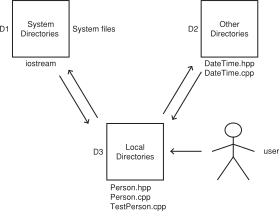
\includegraphics[width=0.4\paperwidth]{./../img/figure2_1}
	\caption{Directory structure for project.}
\end{figure}

\lstinputlisting[
	caption={Hello World class.},
	label=Person.hpp,
]{Person.hpp}

\lstinputlisting[
	caption={Hello World class.},
	label=Person.cpp,
]{Person.cpp}

\lstinputlisting[
	caption={Hello World Testing the first C++ class.},
	label=TestPerson.cpp,
]{TestPerson.cpp}

\lstinputlisting[
	caption={Output of \texttt{TestPerson.cpp}.},
	label=TestPerson.txt,
]{TestPerson.txt}

\section{Template classes and template functions}

\lstinputlisting[
	caption={Header file containing declarations of functions.},
	label=GenericInequalities.hpp,
]{GenericInequalities.hpp}

\lstinputlisting[
	caption={Code file containing declarations of functions.},
	label=GenericInequalities.cpp,
]{GenericInequalities.cpp}

\lstinputlisting[
	caption={Main program (Console-based) to test Max and Min functions.},
	label=TestGenericInequalities.cpp,
]{TestGenericInequalities.cpp}

\section{Kinds of errors}



\subsection{Compiler errors}

\subsection{Linker errors}

\begin{lstlisting}
int age(); // NO "const" in this declaration
\end{lstlisting}

\begin{lstlisting}
int Person::age() const
{
	return int( double(DatasimDate() - dob) / 365.0);
}
\end{lstlisting}

\lstinputlisting[
	caption={Simple stuff for converting built-in types to strings.},
	label=TestConversions.cpp,
]{TestConversions.cpp}

\begin{lstlisting}
#include <string>
#include <cstddef>

stdd::string getString(long j)
{
	char str[200];
	sprintf(str, "%d", j);
	std::string result(str);
	
	return result;
}

stdd::string getString(int j)
{
	char str[200];
	sprintf(str, "%d", j);
	std::string result(str);

	return result;
}

stdd::string getString(size_t j)
{
	char str[200];
	sprintf(str, "%d", j);
	std::string result(str);

	return result;
}
\end{lstlisting}

\subsection{Run-time errors}

\section{The struct concept}

\section{Useful data conversion routines}

\begin{lstlisting}
// Hard-coded example for starters
std::stringstream s;
s << myDouble;
std::string result = s.str();
std::cout << "String value is: " << result << std::endl;
\end{lstlisting}

\begin{lstlisting}
template <typename T>
	std::string getString(const T& value)
{
	stringstream s;
	s << value;
	return s.str();
}
\end{lstlisting}

\section{Summary and conclusions}

\section{Exercises and projects}
% Chapter 3
\chapter{C++ Fundamentals and My First Option Class}

\section{Introduction and objectives}

\section{Class \texttt{==} member data \texttt{+} member functions}

\begin{lstlisting}
ExactEuropeanOption myobject ("P", "Index Option");

// ...

double d = myObject.Price();
\end{lstlisting}

\section{The header file (function prototypes)}

\lstinputpath{../../src/chapter_3}

\begin{lstlisting}
// EuropeanOption.hpp
class EuropeanOption
{
private:

	void init();	// Initialise all default values
	void copy(const EuropeanOption& o2);
	// "Kernel" functions for option calculations
	double CallPrice() const;
	double PutPrice() const;
	double CallDelta() const;
	double PutDelta() const;

public:
	// Public member data for convenience only
	double r;	// Interest rate
	double sig;	// Volatility
	double K;	// Strike price
	double T;	// Expiry date
	double U;	// Current underlying price
	double b;	// Cost of carry

	string optType;	// Option name (call, put)

public:
// Constructors
EuropeanOption();	// Default call option
EuropeanOption(const EuropeanOption& option2);	// Copy constructor
EuropeanOption (const string& optionType);	// Create option type

// Destructor
virtual ~EuropeanOption();

// Assignment operator
EuropeanOption& operator = (const EuropeanOption& option2);

// Functions that calculate option price and (some) sensitivities
double Price() const;
double Delta() const;

// Modifier functions
void toggle();	// Change option type (C/P, P/C)
};
\end{lstlisting}

\section{The class body (code file)}

\begin{lstlisting}
#include "EuropeanOption.hpp"	// Declaration of functions
#include <cmath>	// For mathematical functions, e.g. std::exp()
\end{lstlisting}

\begin{lstlisting}
double EuropeanOption::PutPrice() const
{
	double tmp = sig * std::sqrt(T);

	double d1 = ( std::log(U/K) + (b + (sig*sig)*0.5) * T) / tmp;
	double d2 = d1 - tmp;

	return (K * exp(-r * T)* N(-d2))  - (U * std::exp((b - r)*T) * N(-d1));
}
\end{lstlisting}

\lstinputlisting[
	caption={European options.},
	label=EuropeanOption.cpp,
]{EuropeanOption.cpp}


\section{Using the class}

\lstinputlisting[
	caption={TestEuropeanOption options.},
	label=TestEuropeanOption.cpp,
]{TestEuropeanOption.cpp}

\lstinputlisting[
	language=bash,
	caption={Output of \texttt{TestEuropeanOption.cpp}.},
	label=TestEuropeanOption.txt,
]{TestEuropeanOption.txt}

\section{Examining the class in detail}

\subsection{Accessibility issues}

\subsection{Using standard libraries}

\subsection{The scope resolution operator ``\texttt{::}''}

\begin{lstlisting}
double EuropeanOption::Price() const
{
	if (optType == "C")
	{
		return CallPrice();
	}
	else
		return PutPrice();
}
\end{lstlisting}

\subsection{Virtual destructor: better safe than sorry}

\begin{center}\itshape
Declare all destructors to be virtual.
\end{center}

\section{Other paradigms}

\lstinputlisting[
	caption={Simple functions for interest rate calculations.},
	label=SimpleBondPricing.hpp,
]{SimpleBondPricing.hpp}

\begin{lstlisting}
double fv2 = Chapter3CPPBook::FutureValue(P, nPeriods, r, freq);
\end{lstlisting}

\begin{lstlisting}
using namespace Chapter3CPPBook;
std::cout << "**Future with " << m << " periods: " << FutureValue(PO, nPeriods, r, m) << std::endl;
\end{lstlisting}

\begin{lstlisting}
// Future value of a sum of money invested today
double FutureValue(double PO, long nPeriods, double r)
{
	double factor = 1.0 + r;
	return PO * power(factor, nPeriods);
}
\end{lstlisting}

\begin{lstlisting}
// Non-recursive function to calculate power of a number.
double power(double d, long n)
{
	if (n == 0) return 1.0;
	if (n == 1) return d;
	double result = d;
	for (long j = 1; j < n; j++)
	{
		result *= d;
	}
	return result;
}
\end{lstlisting}

\begin{lstlisting}
// Handy shorthand synonyms
typdef vector<double> Vector;
\end{lstlisting}

\begin{lstlisting}
// Present Value of a series of future values
double PresentValue(const Vector& Prices, long nPeriods, double r)
{
	// Number of periods MUST == size of the vector
	assert (nPeriods == prices.size());

	double factor = 1.0 + r;

	double PV = 0.0;

	for (long t = 0; t < nPeriods; t++)
	{
		PV += prices[t] / power(factor, t + 1);
	}

	return PV;
}
\end{lstlisting}

\begin{lstlisting}
// Present Value of a series of future values
Vector futureValues(5);	// For five years, calls constructor
for (long j = 0; j < 4; j++)
{	// The first 4 years
		futureValues[j] = 100.0;	// Vector has indexing []
}
futureValues[4] = 1100.0;

int nPeriods = 5;
double r = 0.0625;
std::cout << "**Present value, series: " << PresentValue(futureValues, nPeriods, r) << std::endl;
\end{lstlisting}

\section{Summary and conclusions}

\section{Questions, exercises and projects}

Consider the future value of a sum of money
\begin{itemize}
	\item $P_{n}\coloneqq P_{0}{\left(1+r\right)}^{n}$.
	\item $n$ is the number of periods.
	\item $P_{n}$ is the future value $n$ periods from now.
	\item $P_{0}$ is the original principal.
	\item $r$ is the interest rate per period (decimal form)
\end{itemize}
Future value of an ordinary annuity
\begin{itemize}
	\item $P_{n}\coloneqq A\left[\frac{{\left(1+r\right)}^{n}-1}{r}\right]$.
	\item $A$ is the annuity amount.
	\item $r$ is the interest rate.
	\item $n$ is the number of periods.
\end{itemize}
Simple present values calculations
\begin{itemize}
	\item $PV\coloneqq P_{0}=P_{n}\left[\frac{1}{{\left(1+r\right)}^{n}}\right]$
	\item $P_{n}$ is the future value $n$ periods from now.
	\item $r$ is the interest rate.
	\item $PV$ is the present value.
\end{itemize}
Present value of a series of future values
\begin{itemize}
	\item $PV\coloneqq\sum_{t=1}^{n}\frac{P_{t}}{{\left(1+r\right)}^{t}}$
	\item $P_{t}$ is the value at period $t$ from now.
	\item $r$ is the interest rate.
\end{itemize}
Present value of an ordinary annuity
\begin{itemize}
	\item $PV=A\left\{\frac{1-\frac{1}{{\left(1+r\right)}^{n}}}{r}\right\}$
	\item $A$ is the amount of the annuity
\end{itemize}
Continuous Compounding
\begin{itemize}
	\item $P_{n}\coloneqq P_{0}e^{rn}$.
	\item $r$ is the interest rate.
	\item $P_{0}$ is the original principal.
	\item $n$ is the number of years.
\end{itemize}
$m$--Period Compounding \[ P_{n}=P_{0}{\left(1+\frac{r}{m}\right)}^{mn}. \]
% Chapter 4
\chapter{Creating Robust Classes}

\section{Introduction and objectives}

\section{Call by reference and call by value}

\begin{lstlisting}
double Max(double x, double y)
{
	if (x > y)
		return x;
	return y;
}
\end{lstlisting}

\begin{lstlisting}
dobule d1 = 1.0;
double d2 = - 34536.00;

// Copies of d1 and d2 offered to the function Max()
double result = Max(d1, d2);
std::cout << "Maxvalue is " << result << std::endl;
\end{lstlisting}

\begin{lstlisting}
class SampleClass
{
public:	// For convenience only
	// This data created at compile time
	double contents[100];

public:
	SampleClass(double d)
	{
		for (int i = 0; i < 1000; i++)
		{
			contents[i] = d;
		}
	}
	virtual ~SampleClass()
	{
		std::cout << "SampleClass instancce being deleted\n";
	}
}'
\end{lstlisting}

\begin{lstlisting}
double Sum(SampleClass myClass)
{
	double result = myClass.contents[0];
	for (int i = 1; i < 1000; i ++)
	{
		result += myClass.contents[i];
	}
	return result;
}
\end{lstlisting}

\begin{lstlisting}
SampleClass sc(1.0);
double sum = Sum(sc);
\end{lstlisting}

\begin{lstlisting}
double Sum2(SampleClass & myClass)
{
	double result = myClass.contents[0];
	for (int i = 1; i < 1000; i++)
	{
		result += myClass.contents[i];
	}
	return result;
};
\end{lstlisting}

\begin{lstlisting}
double Sum2(SampleClass* myClass);
\end{lstlisting}

\section{Constant objects everywhere}

\begin{lstlisting}
double Sum3(SampleClass* myClass)
{
	// N.B. not possible to modify myClass
};
\end{lstlisting}

\subsection{Read-only (const) member functions}

\begin{lstlisting}
class Point
{
private:
	void init(double xs, double ys);

	// Properties for x- and y-coordinates
	double x;
	double y;

public:

	// Constructors and destructor
	Point();	// Default constructor
	Point(double xs, double ys);	// Construct with coordinates
	Point(const Point& source);	// Copy constructor
	virtual ~Point();

	// Selectors
	double X() const;	// Return x
	double Y() const;	// Return y
	// ...
};
\end{lstlisting}

\begin{lstlisting}
double Point::X() const
{// Return x
		return x;
}

double Point::Y() const
{// Return y
		return y;
}
\end{lstlisting}

\begin{lstlisting}
// Modifiers
void X(double NewX);	// Set x
void Y(double NewY);	// Set y
\end{lstlisting}

\begin{lstlisting}
// Modifiers
void Point::X(double NewX)
{// Set x
		x = NewX;
}

void Point::Y(double NewY)
{// Set y
y = NewY;
}
\end{lstlisting}

\begin{lstlisting}
Point p1(1.0, 3.14);

// Read the coordinate onto the Console
std::cout << "First coordinate: " << p1.X() << std::endl;
std::cout << "Second coordinate: " << p1.Y() << std::endl;

// Modify coordinates
p1.X(2.0);
p1.Y(5.0);

// Read the coordinate onto the Console
std::cout << "First coordinate: " << p1.X() << std::endl;
std::cout << "Second coordinate: " << p1.Y() << std::endl;
\end{lstlisting}

\section{Constructors in detail}

\begin{lstlisting}
Point::Point()
{// Default constructor

	init(0.0, 0.0);
}

Point::Point(double xs, double ys)
{	// Normal constructor with coordinates

		init(xs, ys);
}

Point::Point(const Point &source)
{	// Copy constructor

		init(source.x, source.y);
}
\end{lstlisting}

\begin{lstlisting}
void Point::init(double xs, double ys)
{	/// Initialize the point

		x = xs;
		y = ys;
}
\end{lstlisting}

\begin{lstlisting}
Point();	// Default constructor
Point(const Point& source);	// Copy constructor
\end{lstlisting}

\begin{lstlisting}
Point p1(1.0, 3.14);
Point p2(p1);
Point p3;
\end{lstlisting}

\subsection{Member initialisation}

\begin{lstlisting}
Point::Point(double newx, double newy)
{	// Initialize using newx and newy
		init(newx, newy);
}

Point::Point(double newx, double newy) : x(newx), y(newy)
{	// Initialize using newx and newy
		// init(newx, newy); NOT NEEDED
}
\end{lstlisting}

\section{Static member data and static member functions}

\begin{lstlisting}
class Point: public Shape
{
private:

	// Properties for x- and y-coordinates
	double x;
	double y;

	static Point OriginPoint;

public:

	// Other members
};
\end{lstlisting}

\begin{lstlisting}
Point Point::OriginPoint = Point(0.0, 0.0);
\end{lstlisting}

\begin{lstlisting}
// Accessing the "global" object
statics Point& GetOriginPoint();
\end{lstlisting}

\begin{lstlisting}
Point& Point::GetOriginPoint()
{
	return OriginPoint;
}
\end{lstlisting}

\begin{lstlisting}
// Work with unique Origin Point
std::cout << "Origin point: " << Point::GetOriginPoint() << std::endl;

// Now choose new coordinates for the new origin
Point::GetOriginPoint() = Point(1.0, 2.0);
std::cout << "Origin point: " << Point::GetOriginPoint() << std::endl;
\end{lstlisting}

\section{Function overloading}

\begin{lstlisting}
Point();	// Default constructor
Point(double xs, double ys);	// Construct with coordinates
Point(const Point& source);	// Copy constructor
\end{lstlisting}

\section{Non-member functions}

\section{Performance tips and guidelines}

\subsection{The ``inline'' keyword}

\begin{lstlisting}
double X() const{return x;}
double Y() const{return y;}
\end{lstlisting}

\begin{lstlisting}
inline double X() const{return x;}
inline double Y() const{return y;}
\end{lstlisting}

\subsection{Anonymous objects in function code}

\begin{lstlisting}
Pount MidPoint(const Point& p2) const;
\end{lstlisting}

\begin{lstlisting}
Point Point::MidPoint(const Point& p2) const
{	// Calculate the point between the two points

		Point result((x + p2.x)*0.5, (y + p2.y)*0.5);
		return result;
}
\end{lstlisting}

\begin{lstlisting}
Point Point::MidPoint(const Point& p2) const
{	// Calculate the point between the two points

		// Create "any old" point
		return Point( (x + p2.x)*0.5, (y + p2.y)*0.5);
}
\end{lstlisting}

\begin{lstlisting}
Point pL(0.0, 0.0);
Point pU(1.0, 1.0);

Point pM = pL.MidPoint(pU);
std::cout << "Midpoint: " << pM << std::endl;
\end{lstlisting}

\begin{lstlisting}
Point pM2 = pL.MidPoint(Point(1.0, 1.0));
std::cout << "Midpoint: " << pM2 << std::endl;
\end{lstlisting}

\subsection{Loop optimization}

\section{Summary and conclusions}

\section{Questions, exercises and projects}

\begin{lstlisting}
// Incorrect example
int& FlunkyFunc()
{
	int result = 1;
	std::cout << "Funny";
	return result;
}
\end{lstlisting}

\begin{lstlisting}
FlunkyFunc() = 12;
std::cout << FlunkyFunc() << "eee";
\end{lstlisting}

\begin{lstlisting}
double& WrongFunction()
{
	double d = 3.1415; return d;
}
\end{lstlisting}

\begin{lstlisting}
Point pt; std::cout << "wrong" << pt.WrongFunction() << std::endl;
\end{lstlisting}

\lstinputpath{../../src/chapter_4}

\lstinputlisting[
	caption={Line segments in two dimensions.},
	label=LineSegment.hpp,
]{LineSegment.hpp}
% Chapter 5
\chapter{Operator Overloading in C++}

\section{Introduction and objectives}

\begin{lstlisting}
Complex z1(-23.0, 5.3);
Complex z2(2.0, 3.0);
Complex z3 = z1 * z2;
Complex z4 = 2.0 * z4;
Complex z5 = - z3;
\end{lstlisting}

\section{What is operator overloading and what are the possibilities?}

\begin{lstlisting}
+	-	*	/	%	^	&	|	~
~	=	<	>	<=	>=	==	+=	-=
/=	++	--	!=	&&	>>	<<	&=	<<=
>>=	^=	()	[]	new	delete
\end{lstlisting}

\begin{lstlisting}
x + y
os << "help";	// Using the operator <<
a % b
\end{lstlisting}

\begin{lstlisting}
Complex z6 = z12* 2.0;
Complex z7 = 2.0 * z2;
Complex z8 = z6 * z7;;
\end{lstlisting}

\begin{lstlisting}
Matrix m1(100, 50);	// A matrix with 100 rows and 50 columns
Matrix m2 = m1;	// A new matrix of same size as m1
\end{lstlisting}

\begin{lstlisting}
b = -a;	// b is the negative of a
b++;	// Postfix incremenet
++a;	// Prefix incremeent
\end{lstlisting}

\section{Why use operator overloading? The advantages}

\begin{lstlisting}
Matrix m3 = m1 * m2;
Matrix m4 = m1.Add(m2);
\end{lstlisting}

\begin{lstlisting}
DatasimDate fixed(1, 1, 94);
DatasimDate current(1, 1, 94);
int interval = 30;

for (int j = 0; i < 12; j++)
{
	current = fixed - (j*interval);
	std::cout << current << std::endl;
}
\end{lstlisting}

\begin{lstlisting}
1/1/94, 2/12/93, 2/11/93, 3/10/93, 3/9/93, 4/8/93
5/7/93, 5/6/93, 6/5/93, 6/4/93, 7/3/93, 5/2/93
\end{lstlisting}

\begin{lstlisting}
// Ofsets; quarters + half years
std::cout << "Offset stuff\n";
DatasimDate today;
DatasimDate d3 = today.add_quarter();
DatasimDate d4 = today.add_halfyear();

std::cout << d3 << std::endl;
std::cout << d4 << std::endl;

d3 = d3.sub_quarter();
d4 = d4.sub_quarter();

std::cout << d3 << std::endl;
std::cout << d4 << std::endl;
\end{lstlisting}

%TODO: Offset stuff

\begin{lstlisting}
Vector cross(const Vector& vec) const;	// Cross product
Vector operator ^ (const Vector& vec) const;	// Cross product

double dot(cont Vector& vec) const;	// Dot product
double operator % (const Vector& vec) const;	// Dot product
\end{lstlisting}

\begin{lstlisting}
Vector Vector::vtproduct(const Vector& B, const Vector& C) const
{	// Vector triple product A X (B X C)

	// Schaum Vectors page 17

	Vector tmp = B ^ C;
	return (*this) ^ tmp;
}

double Vector::stprodcut(const Vector& B, const Vector& C) const
{// Scalar triple prodcut A . (B X C)

		// Schaum Vectors, page 17
		Vector tmp = B ^ C;	// Cross
		return (*this) % tmp;	// Dot
}
\end{lstlisting}

\begin{lstlisting}
class Plane
{	// A class for a plane in three dimensions
private:

	Vector n;	// Normal unit vector to plane
	Point p;	// Point on plane
};
\end{lstlisting}

\begin{lstlisting}
Point Plane::closest(const Point& pt) const
{	// The point on plane closest to the point pt
		// GEMS IV page 154
		double d = n % (p - pt);
		Point result = pt + (n.componenets() * d);
		return result;
}
\end{lstlisting}

\section{Operator overloading: the steps}

\begin{lstlisting}
Complex add (const Complex& c2) const;
\end{lstlisting}

\begin{lstlisting}
Complex Complex:: add(const Complex& c2) const
{	// Add two complex numbers

	Complex result;
	result.x = x + c2.x;
	result.y = y + c2.y;

	return result;
}
\end{lstlisting}

\begin{lstlisting}
Complex z3 = z1.add(z2);
\end{lstlisting}

\begin{lstlisting}
Complex operator + (const Complex& c2) const;
\end{lstlisting}

\begin{lstlisting}
Complex Complex::operator + (const Complex& c2) const
{	// Add two complex numbers
	Complex result;
	result.x = x + c2.x;
	result.y = y + c2.y;

	return result;
}
\end{lstlisting}

\begin{lstlisting}
Complex Complex::operator + (const Complex& c2) const
{	// Add two complex numbers

		return Complex(x + c2.x, y + c2.y);
}
\end{lstlisting}

\begin{lstlisting}
Complex operator - (const Complex& c2) const;
Complex operator * (const Complex& c2) const;
Complex operator / (const Complex& c2) const;
\end{lstlisting}

\begin{lstlisting}
Complex z2(2.0, 3.0);

Complex z7 = 2.0 * z2;
Complex z8 = z2 * 2.0;
\end{lstlisting}

\begin{lstlisting}
friend Complex operator * (const Complex& c, double d);
friend Complex operator * (double d, const Complex& c);
\end{lstlisting}


\begin{lstlisting}
Complex operator * (const Complex & c, double d)
{	// Scaling by a double

		return Complex(c.x * d, c.y * d);
}

Complex operator * (double d, const Complex& c)
{	// Scaling by a double
		// Reuse already made operator
		return c * d;
}
\end{lstlisting}

\subsection{A special case: the assignment operator}

\begin{lstlisting}
Complex z7 = z2;
\end{lstlisting}

\begin{lstlisting}
Complex& operator = (const Complex& c);
\end{lstlisting}

\begin{lstlisting}
Complex& Complex::operator = (const Complex& c)
{
		// Avoid doing assign to myself
		if (this == &c)
			return *this;
			
		x = p.x;
		y = p.y;

		return *this;
}
\end{lstlisting}

\begin{lstlisting}
Complex z0(1.0, 2.0);
Complex z1, z2, z3, z4;
z4 = z3 = z1 = z0;
std::cout << "Chain: " << z0 << z1 << z3 << z4;
\end{lstlisting}

\begin{lstlisting}
+=, *=, -=, /=
\end{lstlisting}

\begin{lstlisting}
z4 += z1;	// Multiply z4 by z1 and modify it
\end{lstlisting}

\begin{lstlisting}
Complex& operator += (const Complex& c);
\end{lstlisting}

\begin{lstlisting}
Complex& Complex::operator += (const Complex & c)
{
	x += c.x;
	y += c.y;

	return *this;
}
\end{lstlisting}

\section{Using operator overloading for simple I/O}

\begin{lstlisting}
#include <iostream>
using namespace std;
\end{lstlisting}

\begin{lstlisting}
double real;
double imaginary;
cout << "Creating a complex number" << endl;
cout << "Give real part: ";
cin >> real;
cout << "Give imaginary part: ";
cin >> imaginary;

// User-defined class and putput for its objects
Complex c(real, imaginary);
cout << c;
\end{lstlisting}

\begin{lstlisting}
friend ostream& operator << (ostream& os, const Complex& cmp);
\end{lstlisting}

\begin{lstlisting}
osteam& operator << (ostream& os, const Complex& cmp)
{	// Print the complex number

		os << "(" << cmp.x << ", " << cmp.y << ")\n";
		return os;
}
\end{lstlisting}

\begin{lstlisting}
cout << "First: " << z1 << "Second: " << z2 << endl;
\end{lstlisting}

\section{Friend functions in general}

\begin{lstlisting}
friend Complex exp(const Complex& c);	// Exponential
friend Complex cos(const Complex& c);	// Cosine function
friend Complex sin(const Complex& c);	// Sine function
friend Complex cosh(const Complex& c);	// Hyperbolic  cosine
friend Complex sinh(const Complex& c);	// Hyperbolic sine
\end{lstlisting}

\begin{lstlisting}
Complex exp(const Complex& c)
{	// Exponential function
		double ex = std::exp(c.x);
		return Complex(ex * cos(c.y), ex * sin(c.y));
}
\end{lstlisting}

\begin{lstlisting}
Complex cosh(const Complex& z)
{	// Hyperbolic cosine function
		return (exp(z) + exp(- (z))) * 0.5;
}

Complex cotanh(const Complex& z)
{	// Hyperbolc cotangent
		return cosh(z) / sinh(z);
}
\end{lstlisting}

\begin{lstlisting}
Complex za = exp(Complex(0.0, 0.0));
cout << za;

Complex zs = sinh(za);
Complex zc = cosh(za);

cout << zs << zc;
Complex c2(0.0, 0.0);
cout << sinh(c2) << cosh(c2);
\end{lstlisting}

\subsection{Friend classes}

\begin{lstlisting}
class A
{
private: // Don’t tell others who my friends are
friend class B; // Hi B class, you my friend

// ...
};
\end{lstlisting}



\section{Summary and conclusions}

\section{Exercise}

\lstinputpath{../../src/chapter_5}

\lstinputlisting[
	caption={Testing complex numbers.},
	label=TestComplex.hpp,
]{TestComplex.cpp}

We concentrate on one-dimensional and two-dimensional data structures. To this end, we introduce basic \textit{foundation} classes, namely:

\begin{itemize}
	\item \texttt{Array}: sequential, indexible container containing arbitrary data types.
	\item \texttt{Vector}: array class that contains numeric data.
	\item \texttt{Matrix}: sequential, indexible container containing arbitrary data types.
	\item \texttt{NumericMatrix}: matrix class that contains numeric data.
\end{itemize}
The code for these classes is on the accompanying CD. The classes \texttt{Array} and \texttt{Vector} are one-dimensional containers whose elements we access using a single index while \texttt{Matrix} and \texttt{NumericMatrix} are two-dimensional containers whose elements we access using two indices.

We now discuss each of these classes in more detail.

We start with the class \texttt{Array}. This is the most fundamental class in the library and it
represents a sequential collection of values. This template class that we denote by \texttt{Array<V, I, S>} has three generic parameters:
\begin{itemize}
	\item V: the data type of the underlying values in the array.
	\item I: the data type used for indexing the values in the array (integral).
	\item S: the so-called storage class for the array.
\end{itemize}
The \textit{storage class} is in fact an encapsulation of the STL vector class and it is here that the data in the array is actually initialised. At the moment there are specific storage classes, namely \texttt{FullArray<V>} and \texttt{BandArray<V>} that store a full array and a banded array of values, respectively.

Please note that it is \textbf{not} possible to change the size of an \texttt{Array} instance once it has been constructed. This is in contrast to the STL vector class where it is possible to let it grow.

The declaration of the class \texttt{Array} is given by:

The declaration of the class Array is given by:
\begin{lstlisting}
template <class V, class I = int, class S = FullArray<V> >
class Array
{
private:
	S m_structure; // The array structure
	I m_start; // The start index
};
\end{lstlisting}

We see that \texttt{Array} has an embedded storage object of type $S$ and a start index. The default storage is \texttt{FullArray<V>} and the default index type is \texttt{int}. This means that if we work with these types on a regular basis that we do not have to include them in the template declaration.

Thus, the following three declarations are the same:
\begin{lstlisting}
Array<double, int, FullArray<double> > arr1;
Array<double, int> arr1;
Array<double> arr1;
\end{lstlisting}

You may choose whichever data types that are most suitable for your needs.

The constructors in \texttt{Array} allow us to create instances based on size of the array, start index and so on. The constructors are:

\begin{lstlisting}
Array();	// Default constructor
Array(size t size);	// Give length start index ==1
Array(size t size, I start);	// Length and start index
Array(size t size, I start, const V& value);	// Size, start, value
Array(const Array<V, I, S>& source);	// Copy constructor
\end{lstlisting}

Once we have created an array, we may wish to navigate in the array, access the elements in the array and to modify these elements. The member functions to help you in this case are:
\begin{lstlisting}
// Selectors
I MinIndex() const;	// Return the minimum index
I MaxIndex() const;	// Return the maximum index
size t Size() const;	// The size of the array
const V& Element(I index) const;	// Element at position

// Modifiers
void Element(I index, const V& val);	// Change element at position
void StartIndex(I index);	// Change the start index

// Operators
virtual V& operator [] (I index);	// Subscripting operator
virtual const V& operator [] (I index) const;
\end{lstlisting}
This completes the description of the \texttt{Array} class. We do not describe the class that actually stores the data in the array. The reader can find the source code on the accompanying media kit. We now discuss the \texttt{Vector} and \texttt{NumericMatrix} classes in detail. These classes are derived from \texttt{Array} and \texttt{Matrix}, respectively. Furthermore, we have created constructors for \texttt{Vector} and \texttt{NumericMatrix} classes as well. So what have these classes got that their base classes do
not have? The general answer is that \texttt{Vector} and \texttt{NumericMatrix} assume that their underlying types are numeric. We thus model these classes as implementations of the corresponding mathematical structures, namely \textit{vector space} and, \textit{inner product} spaces.

We have implemented \texttt{Vector} and \texttt{NumericMatrix} as approximations to a vector space. In some cases we have added functionality to suit our needs. However, we have simplified things a little because we assume that the data types in a vector space are of the same types as the underlying field. This is for convenience only and it satisfies our needs for most applications in financial engineering.

Class \texttt{Vector} is derived from \texttt{Array}. Its definition in C++ is:

\begin{lstlisting}
template <class V, class I=int, class S=FullArray<V> >
class Vector: public Array<V, I, S>
{
private:
	// No member data
};
\end{lstlisting}

We give the prototypes for some of the mathematical operations in \texttt{Vector}. The first is a straight implementation of a vector space; notice that we have applied operator overloading in C++:

\begin{lstlisting}
Vector<V, I, S> operator - () const;
Vector<V, I, S> operator + (const Vector<V, I, S>& v) const;
Vector<V, I, S> operator - (const Vector<V, I, S>& v) const;
\end{lstlisting}
The second group of functions is useful because it provides functionality for \textit{offsetting} the values in a vector:
\begin{lstlisting}
Vector<V, I, S> operator + (const V& v) const;
Vector<V, I, S> operator - (const V& v) const;
Vector<V, I, S> operator * (const V& v) const;
\end{lstlisting}
The first function adds an element to each element in the vector and returns a new vector. The second and third functions are similar except that we apply subtraction and multiplication operators.

Class \texttt{NumericMatrix} is derived from \texttt{Matrix}. Its definition in C++ is:

\begin{lstlisting}
template <class V, class I=int, class S=FullMatrix<V> >
class NumericMatrix: public Matrix<V, I, S>
{
private:
	// No member data
};
\end{lstlisting}
The constructors in \texttt{NumericMatrix} are the same as for \texttt{Matrix}. We may also wish to manipulate the rows and columns of matrices to this end to provide ``set/get'' functionality. Notice that we return vectors for selectors but that modifiers accept \texttt{Array} instances (and instances of any derived class!):

\begin{lstlisting}
// Selectors
Vector<V, I> Row(I row) const;
Vector<V, I> Column(I column) const;

// Modifiers
void Row(I row, const Array<V, I>& val);
void Column(I column, const Array<V, I>& val);
\end{lstlisting}
Since we will be solving linear systems of equations in later chapters we must provide functionality for multiplying matrices with vectors and with other matrices:
\begin{itemize}
	\item Multiply a matrix and a vector.
	\item Multiply a (transpose of a) vector and a matrix.
	\item Multiply two matrices
\end{itemize}
Notice that the last two functions are not member of \texttt{NumericMatrix} but are non-member friends. This ploy allows us to multiply a matrix by a vector or vice versa.

We give some simple examples showing how to create vectors and how to perform some mathematical operations on the vectors.

\begin{lstlisting}
// Create some vectors
Vector<double, int> vec1(10, 1, 2.0);	// Start = 1, value 2.0
Vector<double, int> vec2(10, 1, 3.0);	// Start = 1, value 3.0

Vector<double, int> vec3 = vec1 + vec2;
Vector<double, int> vec4 = vec1 - vec2;

Vector<double, int> vec5 = vec1 - 3.14;
\end{lstlisting}
We give an example to show how to use numeric matrices. The code is:
\begin{lstlisting}
int rowstart = 1;
int colstart = 1;
NumericMatrix<double, int> m3(3, 3, rowstart, colstart);
for (int i = m3.MinRowIndex(); i <= m3.MaxRowIndex(); i++)
{
}
	for (int j = m3.MinColumnIndex(); j <= m3.MaxColumnIndex(); j++)
	{
		m3(i, j) = 1.0 /(i + j -1.0);
	}
print (m3);
\end{lstlisting}

\begin{lstlisting}
MinRowIndex: 1 , MaxRowIndex: 3
MinColumnIndex: 1 , MaxColumnIndex: 3
MAT:[
Row 1 (1,0.5,0.333333,)
Row 2 (0.5,0.333333,0.25,)
Row 3 (0.333333,0.25,0.2,)]
\end{lstlisting}
% Chapter 6
\chapter{Memory Management in C++}

\section{Introduction and objectives}

\section{Single objects and arrays of objects on the stack}

\begin{lstlisting}
int main()
{
	{	// Define a scope
		int j = 2;
		cout << j << endl;
	}

	cout << j;

	return 0;
}
\end{lstlisting}

\begin{lstlisting}
int myArr[10];

// Initialise the array
for (int j = 0; j < 10; j++)
{
		myArr[j] = j + 1;
		cout << myArr[j] << ",";
}
\end{lstlisting}

\begin{lstlisting}
cout << endl << myArr[-1];
cout << endl << myArr[1000];
\end{lstlisting}

\begin{lstlisting}
class SimpleOption
{
public:
		double T;
		double K;
		// ...

		SimpleOption () { T = 1.0; K = 100.0; }

	void print() const
	{	// Read contents of option

	cout << "Expiry: "<< T << ", " << "Strike: " << K;
	}
};
\end{lstlisting}

\begin{lstlisting}
{	// Define a scope

		SimpleOption opt1;
		opt1.print();
}
\end{lstlisting}

\begin{lstlisting}
SimpleOption myPortfolio[10];

// Initialise the array
for (int j = 0; j < 10; j++)
{
	myPortfolio[j].print();
}
\end{lstlisting}

\begin{lstlisting}
myPortfolio[-1].print();
myPortfolio[1000].print();
\end{lstlisting}

\section{Special operators: ``\texttt{new}'' and ``\texttt{delete}''}

\subsection{Single objects}

\begin{lstlisting}
SimpleOption* opt;
SimpleOption* opt2;
\end{lstlisting}

\begin{lstlisting}
// Call default constructor
opt = new SimpleOption;
opt -> print();
\end{lstlisting}

\begin{lstlisting}
(* opt).print();
// Call constructor with 2 parameters
opt2 = new SimpleOption(0.25, 90.0);
opt2 -> print();
\end{lstlisting}

\begin{lstlisting}
delete opt;
delete opt2;
\end{lstlisting}

\begin{lstlisting}
opt = new SimpleOption;
(* opt).print();
delete opt;
\end{lstlisting}

\subsection{Arrays of objects}

\begin{lstlisting}
// Now create an array of options
SimpleOption* optArray;
\end{lstlisting}

\begin{lstlisting}
const int N = 10;
optArray = new SimpleOption[N]; // Default constructor called
\end{lstlisting}

\begin{lstlisting}
for (int j = 0; j < N; j++)
{ // Member data public for convenience only
	optArray[j].T = 1.0; // 1 year expiry
	optArray[j].K = 100.0; // Strike price
	optArray[j].print();
}
\end{lstlisting}

\begin{lstlisting}
delete [] optArray;
\end{lstlisting}

\section{Small application: working with complex numbers}

\begin{lstlisting}
Complex myFunc(const Complex& z)
{ // Single valued function of a complex variable
}
return z * z;
\end{lstlisting}

\begin{lstlisting}
Complex z1(1.0, 1.0);
Complex z2(2.0, 3.0);

Complex z3 = z1 * z2;
Complex z4 = 2.0 * z3;
Complex z5 = - z3;

// Create a dynamic list of Complex numbers
int Size = 5;
Complex* cpArray = new Complex[Size];
cpArray[0] = z1;
cpArray[1] = z2;
cpArray[2] = z3;
cpArray[3] = z4;
cpArray[4] = z5;
\end{lstlisting}

\begin{lstlisting}
// Call function and print values for each z
for (int j = 0; j < Size; j++)
{
		cout << myFunc(cpArray[j]) << ", ";
}

delete [] cpArray;
\end{lstlisting}

\begin{lstlisting}
Complex ComplexProduct(Complex* carr, int n)
{ // Complex function of several complex variables
	Complex product = carr[0];

	for (int j = 1; j < n; j++)
	{
		product * = carr[j];
	}

	return product;

}

Complex ComplexSum(Complex* carr, int n)
{ // Complex function of several complex variables

	Complex sum = carr[0];

	for (int j = 1; j < n; j++)
	{
		sum += carr[j];
	}

	return sum;

}
\end{lstlisting}

\begin{lstlisting}
const int N = 5;
Complex fixedArray[5]; // The constant "5" is mandatory
for (int i = 0; i < Size; i++)
{
		fixedArray[i] = Complex ((double) i, 0.0);
}
\end{lstlisting}

\begin{lstlisting}
Complex product = ComplexProduct(fixedArray, Size);
cout << "Product: " << product << endl;

Complex sum = ComplexSum(fixedArray, Size);
cout << "Sum: " << sum << endl;
\end{lstlisting}

\section{Creating an array class}

\subsection{Memory allocation and deallocation}

\begin{lstlisting}
private:
	Complex* arr;
	int size;
\end{lstlisting}

\begin{lstlisting}
ComplexArray(int size);
ComplexArray(const ComplexArray& source);
\end{lstlisting}

\begin{lstlisting}
// Constructor with size
ComplexArray::ComplexArray(int Size)
{
	arr=new Complex[size];
	size=Size;
}

// Copy constructor
ComplexArray::ComplexArray(const ComplexArray& source)
{
	// Deep copy source
	size=source.size;
	arr=new Complex[size];
	for (int i=0; i<size; i++) arr[i]=source.arr[i];
}
\end{lstlisting}

\begin{lstlisting}
virtual ∼ComplexArray();
\end{lstlisting}

\begin{lstlisting}
ComplexArray::∼ComplexArray()
{
	delete[] arr;
}
\end{lstlisting}

\subsection{Accessing functions}

\begin{lstlisting}
int MinIndex() const; // Smallest index in array
int MaxIndex() const; // Largest index in array
\end{lstlisting}

\begin{lstlisting}
const Complex& operator[](int index) const;
Complex& operator[](int index);
\end{lstlisting}


\begin{lstlisting}
Complex ComplexSum(const ComplexArray& carr, int n)
{	// Complex function of several complex variables

		Complex sum = carr[carr.MinIndex()];

		for(int j = carr.MinIndex() + 1; j <= carr.MaxIndex(); j++)
		{
			sum += carr[j];
		}
		return sum;
}
\end{lstlisting}

\subsection{Examples}

\begin{lstlisting}
ComplexArray fixedArray(5);
for (int i=fixedArray.MinIndex();i<=fixedArray.MaxIndex(); i++)
{
	fixedArray[i] = Complex ((double) i, 0.0);
}
\end{lstlisting}

\subsection{The full header file}

\lstinputpath{../../src/chapter_6}

\lstinputlisting[
	caption={Simple Complex Array class.},
	label=ComplexArray.hpp,
]{ComplexArray.hpp}

\section{Summary and conclusions}

\section{Exercises}

\begin{lstlisting}
// Compile-time
Complex matrix [10][20];

// Run-time (pointers to pointers)
Complex** matrix2;

// "Hybrid": pointers to fixed arrays
Complex* matrix3[10];
\end{lstlisting}

\begin{lstlisting}
void MySwap(Complex c1, Complex c2); // Call by value
void MySwap2(Complex& c1, Complex& c2); // Call by reference
void MySwap3(const Complex& c1, const Complex& c2); // const references
void MySwap4(Complex* c1, Complex* c2); // Using pointers
void MySwap5(const Complex* c1, const Complex* c2); // const pointers
\end{lstlisting}

\begin{lstlisting}
struct Point
{
	double x;	// x coordinate
	double y;	// y coordinate
}
\end{lstlisting}

\begin{lstlisting}
class Stack
{
private:

		// EXX What is the member data in this case?

		Stack(const Stack& source);	// Copy constructor
		// Operators
		Stack& operator = (const Stack& source);

public:
		// Constructors & destructor
		Stack();	// Default constructor
		Stack(int NewSize);	// Initial size of the stack

		void Push(double NewItem);	// Push element onto stack
		double Pop();	// Pop last pushed element
};

#endif // STACK HPP
\end{lstlisting}

\begin{lstlisting}
#include <iostream>
using namespace std;

int main()
{
	double m[10][20];

	m[0][1] = 2.0;

	// etc.

	cout << m[0][1] << endl;

	return 0;
}
\end{lstlisting}

\section{Review questions and comments}

\begin{lstlisting}
double mat[10][20];
\end{lstlisting}
% Chapter 7
\chapter{Functions, Namespaces and Introduction to Inheritance}

\section{Introduction and objectives}

\section{Functions and function pointers}

\subsection{Functions in financial engineering}

\subsection{Function categories}

A common notation for a function $f$ from $D$ to $R$ is \[ f\colon D\rightarrow R. \] Functions can be composed. For example, suppose $f$ is a mapping from $D$ to $R1$ and $g$ is a mapping from $R_{1}$ and $g$ is a mapping from $R1$ to $R2$ then the composition of $g$ and $f$ is defined by \[ \left(gf\right)\left(x\right)=g\left(f\left(x\right)\right)\text{ for all }x\text{ in }D. \] Notice that the range of the composed mapping $gf$ is $R2$.

\begin{lstlisting}
void genericFunction (double myX, double myY, double (* f) (double x, double y))
{

	// Call the function f with arguments myX and myY
	double result = (* f)(myX, myY);

	cout << "Result is: " << result << endl;
}
\end{lstlisting}

\begin{lstlisting}
double add(double x, double y)
{
	cout << "** Adding two numbers: " << x << ", " << y << endl;
	return x + y;
}
double multiply(double x, double y)
{
	cout << "** Multiplying two numbers: " << x << ", " << y << endl;
	return x * y;
}
double subtract(double x, double y)
{
	cout << "** Subtracting two numbers: " << x << ", " << y << endl;
	return x - y;
}
\end{lstlisting}

\subsection{Modelling functions in C++}

\begin{lstlisting}
int main()
{
	double x = 3.0;
	double y = 2.0;
	genericFunction(x, y, add);
	genericFunction(x, y, multiply);
	genericFunction(x, y, subtract);

	return 0;
}
\end{lstlisting}

\subsection{Application areas for function pointers, part I}

\section{An introduction to namespaces in C++}

\begin{lstlisting}
namespace MyFunctions
{
	double diffusion (double x) { return x; }
	double convection (double x) { return x* x; }
}
namespace YourFunctions
{
	double diffusion (double x) { return 2.0; }
	double convection (double x) { return 1.0; }
}
\end{lstlisting}

\begin{lstlisting}
cout << YourFunctions::convection (10.0) << endl;
\end{lstlisting}

\begin{lstlisting}
using YourFunctions::convection;
cout << convection (10.0) << endl;
\end{lstlisting}

\begin{lstlisting}
using namespace MyFunctions;
cout << "Directive: \ n";
cout << convection (10.0) << endl;
cout << diffusion (2.0) << endl;
\end{lstlisting}

\begin{lstlisting}
using namespace YourFunctions;
cout << convection (10.0) << endl;
cout << diffusion (2.0) << endl;
\end{lstlisting}

\subsection{Some extra functionality}

\begin{lstlisting}
namespace YA = YourFunctions; // Define alias NS called YA
cout << YA::diffusion (2.0) << endl;
\end{lstlisting}

\begin{lstlisting}
namespace StandardInterface
{
	// Namespace consisting of function pointers
	double (* func1) (double x);
	double (* func2) (double x, double y);
}
\end{lstlisting}

\begin{lstlisting}
namespace Implementation1
{
	double F1 (double x) { return x; }
	double F2 (double x, double y) { return x* y; }
}

namespace Implementation2
{
	double G1 (double x) { return -x; }
	double G2 (double x, double y) { return -x* y; }
}
\end{lstlisting}

\begin{lstlisting}
// Assign the function pointers from NS
StandardInterface::func1 = Implementation1::F1;
StandardInterface::func2 = Implementation1::F2;
\end{lstlisting}

\begin{lstlisting}
using namespace StandardInterface;
cout << func1(2.0) << ", " << func2(3.0, -4.0) << endl;
\end{lstlisting}

\begin{lstlisting}
func1 = Implementation2::G1;
func2 = Implementation2::G2;
cout << func1(2.0) << ", " << func2(3.0, -4.0) << endl;
\end{lstlisting}

\section{An introduction to the inheritance mechanism in C++}

\begin{lstlisting}
class Person
{
public: // Everything public, for convenience only
	// Data
	string nam;	// Name of person
	DatasimDate dob;	// Date of birth
	DatasimDate createdD;	// Internal, date created
	DatasimDateTime createdT;	// Internal, time created
public:
	// Public functions
};
\end{lstlisting}

\begin{lstlisting}
Person (const string& name, const DatasimDate& DateofBirth)
{
	nam = name;
	dob = DateofBirth;
	createdD = DatasimDate();	// default, today REALLY!
	createdT = DatasimDateTime();	// default, now REALLY!
}
\end{lstlisting}

\begin{lstlisting}
void print() const
{
// Who am I?
	cout << "\ n** Person Data ** \ n";
	cout << "Name: " << nam << "Date of birth: " << dob
		<< ", Age: " << age() << endl;
	cout << "Object created: " << createdD
		<< " "; createdT.print(); cout << endl;
}
int age() const
{
	return int( double(DatasimDate() - dob) / 365.0);
}
\end{lstlisting}

\begin{lstlisting}
DatasimDate myBirthday(29, 8, 1952);
string myName ("Daniel J. Duffy");
Person dd(myName, myBirthday);
dd.print();

DatasimDate bBirthday(06, 8, 1994);
string bName ("Brendan Duffy");
Person bd(bName, bBirthday);
bd.print();
\end{lstlisting}

\subsection{Basic inheritance structure}

\lstinputpath{../../src/chapter_7}

\lstinputlisting[
	caption={Output of \texttt{Person.cpp}.},
	label=Person.txt,
]{Person.txt}

\begin{lstlisting}
class Employee : public Person
{
public: // For convenience only
	std::string fun; // Function
	double sal; // Salary
	int rAge; // Retirement age
	// other functions
};
\end{lstlisting}

\subsection{Adding new functionality}

\begin{lstlisting}
void print() const
{ // Who am I and what do I do?

// Print Base class data
cout << "\ n** Employee Data ** \ n";
Person::print(); // Call print() in the base class

// Now print data from current derived class
cout << "\ nFunction: " << fun << ", Salary: " << sal
	<< ", Retires at: " << rAge << endl
	<< YearsToRetirement() << " years to retirement.\ n";
}
\end{lstlisting}

\begin{lstlisting}
int YearsToRetirement() const
{ // How many more years slogging away at C++?
	return rAge - age();
}
\end{lstlisting}

\begin{lstlisting}
Employee dde (myName, myBirthday, string("Cuchulainn Chief"), 0.01, 65);
dde.print();
\end{lstlisting}

\lstinputlisting[
	caption={Output of \texttt{TestPersonAndEmployee.cpp}.},
	label=TestPersonAndEmployee.txt,
]{TestPersonAndEmployee.txt}

\subsection{Overriding functionality: polymorphic and non-polymorphic behaviour}

\begin{lstlisting}
Employee dde (myName, myBirthday, string("Cuchulainn"), 0.01, 65);
Person* p = &dde;
p -> print();
\end{lstlisting}

\begin{lstlisting}[language=bash]
** Person Data **
Name: Daniel J. Duffy, Date of birth: 29/8/1952, Age: 52
Object created: 15/4/2005 19:11:32
Working with pointers II
\end{lstlisting}

\begin{lstlisting}
virtual void DeepPrint() const
{
	print(); // Calls Person::print()
}
\end{lstlisting}

\begin{lstlisting}
void DeepPrint() const
{
	print(); // Calls Employee::print()
}
\end{lstlisting}

\begin{lstlisting}
Employee dde (myName, myBirthday, std::string("Cuchulainn Chief"), 0.01, 65);
Person* p = &dde;
p -> DeepPrint();
\end{lstlisting}

\begin{lstlisting}
** Employee Data **
** Person Data **
Name: Daniel J. Duffy, Date of birth: 29/8/1952, Age: 52
Object created: 15/4/2005 19:11:32
Function: Cuchulainn, Salary: 0.01, Retires at: 65
13 years to retirement.
\end{lstlisting}

\begin{lstlisting}
Person* parr[3]; // Array of pointers
parr[0] = new Employee(...);
parr[1] = new TaxPayer(...);
parr[2] = new ShareHolder(...);
// Now print the array
for (int j = 0; j < 3; j++)
{
	parr[j] -> DeepPrint();
}
\end{lstlisting}

\section{Multiple inheritance}

\begin{lstlisting}
class D: public Base1, public Base2
{
	// Members of D here
};
\end{lstlisting}

\begin{lstlisting}
class D : public Base1
{
private:
	Base2* base2;
public:
	// Members here
};
\end{lstlisting}

\section{Solution of nonlinear equations}

In this section we discus the problem of finding real values $x$ that satisft the equation \[ f\left(x\right)=0 \] where $f$ is a real-valued function. The methods to be discussed are:
\begin{itemize}
	\item Bisection method.
	\item Newton's method.
	\item Secant method.
	\item Steffensen iteration
\end{itemize}

The \emph{bisection method} assume that the function $f\left(x\right)$ has a zero in the interval $\left(a,b\right)$ and we assume that the signs are opposite at the end points, that is $f\left(a\right)f\left(b\right)<0$. The essence of the method is to divide the interval into equals parts until we arrive at an interval that is so small that contains the zero of the function and is small enough to satisfy the given tolerance. The basic algorithm is defined using a sequence of intervals of ever-diminishing size: \[ \left(a,b\right)\supset\left(a_{1},b_{1}\right)\supset\left(a_{2},b_{2}\right)\supset\left(a_{3},b_{3}\right)\supset\cdots \] where \[ \left(a_{k},b_{k}\right)=\begin{cases}\left(m_{k},b_{k-1}\right)&\text{if }f\left(m_{k}\right)<0\\\left(a_{k-1},m_{k}\right)&\text{if }f\left(m_{k}\right)>0\end{cases} \] and \[ m_{k}=\frac{1}{2}\left(a_{k-1}+b_{k-1}\right). \] After $n$ steps the root is in an interval having a length given by \[ b_{n}-a_{n}=2^{-1}\left(b_{n-1}-a_{n-1}\right)=2^{-n}\left(b-a\right). \] Thus the deviation from the exact root $\alpha$ is given by \[ \alpha = m_{n+1}\pm d_{n},\quad d_{n}=2^{-n-1}\left(b-a\right). \] In general we are interested in locating the zero of the function to within a given tolerance \texttt{TOL}. This means that we wish to calculate the number of subdivisions of the original interval $\left(a,b\right)$. To this end, some arithmetic based on the equation below give us the following estimate: \[ n>\frac{\log\left(\frac{b-a}{\texttt{TOL}}\right)}{\log2}-1. \] The advantage of the Bisection method is that we always can define an interval of arbitrary size in which the zero is located. The disadvantage is that convergence is slow. In fact, at each step we gain one binary digit in accuracy. We note also that the rate of convergence is independent of the given function $f\left(x\right)$. The method may be used to give us good initial approximations to more sophisticated nonlinear solvers.

Newton's method (or the \emph{Newton-Raphson} method as it is also called) is probably one of the most famous iterative schemes in Numerical Analysis.

The main advantage of the Newton-Raphson method is that it converges quickly. We say thaat its order of convergence is two by which we mean that the error at each iteration decreases quadratically: \[ x_{n+1}=x_{n}+h_{n},\quad h_{n}=-\frac{f\left(x_{n}\right)}{f^{\prime}\left(x_{n}\right)}. \] The disadvantage is that the choice of the initial approximation is vitally important. If this is not chosen carefully the method may not converge at all or it may even converge to the wrong solution. Furthermore, we must have an analytical expression for the derivative of $f$ and this may not always be available.

The \emph{secant method} can be derived from the Newton-Raphson methody by approximating the derivate by a divided difference. The resulting iterative scheme now becomes: \[ x_{n+1}=x_{n}+h_{n},\quad h_{n}=-f_{n}\frac{x_{n}-x_{n-1}}{f_{n}-f_{n-1}},\quad f_{n}\neq f_{n-1}. \] We note that the secant needs two initial approximations in contrast to Newton-Raphson, that only needs one initial approximation. In general, we must be careful when programming the secant method when the function values are close and/or the solutions at levels $n$ and $n+1$ are close; in such cases we calculate terms that effectively $0/0!$

A disadvantage of the secant method is that it is only first-order accurate. In order to achieve second-order accuracy without having to evaluate derivatives we propose \emph{Steffensen's method}, given by the scheme: \[ x_{n+1}=x_{n}-\frac{f\left(x_{n}\right)}{g\left(x_{n}\right)} \] \[ g\left(x_{n}\right)=\frac{f\left(x_{n}+f\left(x_{n}\right)\right)-f\left(x_{n}\right)}{f\left(x_{n}\right)}. \] This scheme requires two function evaluations but no computation of a derivative. With the exception of the bisection method, the choice of the initial approximation is vital and it must be ``close'' to the exact solution, otherwise the iterative scheme may not converge. There are iterative methods based on the continuation (or homotopy) methods that converge to the true solution een when the initial guess is not good, but a discussion of these techniques it outside the scope of this book.

\section{Nonlinear solvers in C++: design and implementation}

\begin{lstlisting}
class NonlinearSolver
{
public:
	double (*myF)(double x);	// Function whose root we want
	double tol;	// Desired accuracy
public:
	NonlinearSolver(double (* function)(double)) { }
	virtual double solve() = 0;
};
\end{lstlisting}

\begin{lstlisting}
class SteffensensSolver : public NonlinearSolver
{ // One-step nonlinear solver
private:
	double x0;	// Initial guess
	double xPrevious, xCurrent;
	long n;	// Number of iterations taken
public:
	SteffensensSolver(double guess, double (* myFunc)(double x))
	{
		x0 = guess; xPrevious = x0;
		myF = myFunc;
	}

double solve()
	{
		double tmp; double hn; n = 1; xPrevious = x0;
L1:
		tmp = myF(xPrevious);
		hn = (myF(xPrevious + tmp) - tmp)/ tmp;
		hn = tmp/hn;
		xCurrent = xPrevious - hn;

		xPrevious = xCurrent;
		n++;
		if (::fabs(hn) <= tol)
		{
			return xCurrent;

		}
		gotoL1;
	}
	void printStatistics() const
	{
		cout << "\ nData pertaining to Steffensen's method\ n";
		}
		cout << "Value: " << xCurrent << endl;
		cout << "Number of iterations (actual): "
		<< n << endl;
	}
};
\end{lstlisting}

\section{Applying nonlinear solvers: calculating volatility}

\begin{lstlisting}
double CallPrice(double sig)
{
	// Test case Haug p. 172; student exercise to extend it
	double S = 59.0;
	double K = 60.0;
	double r = 0.067;
	double marketPrice = 2.82;	// The call price
	double b = r;
	double T = 0.25;	// Three months

	double tmp = sig * sqrt(T);
	double d1 = ( log(S/K) + (b+ (sig* sig)* 0.5 ) * T )/ tmp;
	double d2 = d1 - tmp;

	double calculatedValue = (S * exp((b-r)* T) * N(d1)) - (K * exp(-r * T)* N(d2));

	// Function in the form f(x) = 0
	return marketPrice - calculatedValue;
}
\end{lstlisting}

\begin{lstlisting}
// Steffensen's method
double guess = 0.2;

SteffensensSolver steff(guess, CallPrice);
steff.tol = 0.0001;

double resultST= steff.solve();
cout << "Steffensen's Method: " << resultST << endl;

steff.printStatistics();
\end{lstlisting}

\section{Summary and conclusions}

\section{Exercises and projects}

\[ y=f\left(a\right)+\frac{f\left(a\right)-f\left(b\right)}{a-b}\left(x-a\right) \] giving the estimate for $c$: \[ c = a - \frac{\left(a-b\right)f\left(a\right)}{f\left(a\right)-f\left(b\right)}. \] This all translates to the algorithm: \[ x_{n}=x_{n-1}-\frac{\left(x_{n-1}-x_{n-2}\right)f\left(x_{n-1}\right)}{f\left(x_{n-1}\right)-f\left(x_{n}-2\right)}. \]
% Chapter 8
\chapter{Advanced Inheritance and Payoff Class Hierarchies}

\section{Introduction and objectives}

\section{The \texttt{virtual} specifier and memory deallocation}

\begin{lstlisting}
class B
{ // Class with non-virtual destructor
private:
	double* d;
public:
	B() { d = new double (1.0); }
	∼B() { cout << "Base destructor\ n"; delete d; }
};
\end{lstlisting}

\begin{lstlisting}
class D : public B
{ // Derived class
private:
	int* iarr;
public:
	D(int N) { iarr = new int[N]; }
	∼D() { cout << "Derived destructor\ n"; delete [] iarr; }
};
\end{lstlisting}

\begin{lstlisting}
int main()
{
	{
		B* b = new D(10);
		delete b;
	}

	return 0;
}
\end{lstlisting}

\begin{lstlisting}
virtual ∼B() { cout << "Base destructor\ n"; delete d; }
\end{lstlisting}

\begin{verbatim}
Derived destructor
Base destructor
\end{verbatim}

\section{Abstract and concrete classes}

\begin{lstlisting}
class Payoff
{
public:
	// Constructors and destructor
	Payoff();	// Default constructor
	Payoff(const Payoff& source);	// Copy constructor
	virtual ∼Payoff();// Destructor

	// Operator overloading
	Payoff& operator = (const Payoff& source);

	// Pure virtual payoff function
	virtual double payoff(double S) const = 0; // Spot price S
};
\end{lstlisting}

\begin{lstlisting}
class CallPayoff: public Payoff
{
private:

	double K;	// Strike price

public:
	// Constructors and destructor
	CallPayoff();
	CallPayoff(double strike);
	CallPayoff(const CallPayoff& source);
	virtual ∼CallPayoff();

	// Selectors
	double Strike() const;	// Return strike price

	// Modifiers
	void Strike(double NewStrike);	// Set strike price

	CallPayoff& operator = (const CallPayoff& source);

	// Implement the pure virtual payoff function from base class
	double payoff(double S) const; // For a given spot price
};
\end{lstlisting}

We see that this class has private number data representing the strike price of the call option as well as public set/get member for this data. Furthermore, we have coded all essential functions in this class:
\begin{itemize}
	\item Default constructor.
	\item Copy constructor.
	\item Virtual destructor.
	\item Assigment operator.
\end{itemize}
We call this \emph{canonical header file}. Finally, we must implement the \texttt{payoff()} function, otherwise \texttt{CallPayoff} will itself be an abstract class.
We now examine the bodies of the member functions of \texttt{CallPayoff}. In general, a constructor in a derived class must initialise the local as well as the data in the class that it is derived from. For the former case we use normal assignment but we can also use the so-called colon syntax to initialise the data in a base class. For example, the copy constructor in \texttt{CallPayoff} is given by:

\begin{lstlisting}
CallPayoff::CallPayoff(const CallPayoff& source): Payoff(source)
{ // Copy constructor
	K = source.K;
}
\end{lstlisting}

\begin{lstlisting}
CallPayoff& CallPayoff::operator = (const CallPayoff &source)
{ // Assignment operator

		// Exit if same object
		if (this==&source) return * this;

		// Call base class assignment
		Payoff::operator = (source);

		// Copy state
		K = source.K;

		return * this;
}
\end{lstlisting}

\begin{lstlisting}
double CallPayoff::Strike() const
{
// Return K
	return K;
}

void CallPayoff::Strike(double NewStrike)
{// Set K
	K = NewStrike;
}
\end{lstlisting}

\begin{lstlisting}
double CallPayoff::payoff(double S) const
{ // For a given spot price

	if (S > K)
		return (S - K);
	return 0.0;
	// remark; possible to say max (S - K, 0)if you prefer
}
\end{lstlisting}

\begin{lstlisting}
double BullSpreadPayoff::payoff(double S) const
{ // Based on Hull's book

	if (S >= K2)
		return K2 - K1;
	if (S <= K1)
		return 0.0;

	// In the interval [K1, K2]
	return S - K1;
}
\end{lstlisting}

\subsection{Using payoff classes}

\begin{lstlisting}
CallPayoff call(20.0);

cout << "Give a stock price (plain Call): ";
double S;
cin >> S;

cout << "Call Payoff is: " << call.payoff(S) << endl;
\end{lstlisting}

\begin{lstlisting}
double K1 = 30.0;	// Strike price of bought call
double K2 = 35.0;	// Strike price of sell call
double costBuy = 3.0;	// Cost to buy a call
double sellPrice = 1.0; // Sell price for call
BullSpreadPayoff bs(K1, K2, costBuy, sellPrice);
cout << "Give a stock price (BullSpread): ";
cin >> S;

cout << "Bull Spread Payoff is: " << bs.payoff(S) << endl;
cout << "Bull Spread Profit is: " << bs.profit(S) << endl;
\end{lstlisting}

\begin{lstlisting}
double BullSpreadPayoff::profit(double S) const
{ // Profit
	return payoff(S) - (buyValue - sellValue);
}
\end{lstlisting}
The techniques developed in this section can be used in other applications in which we need to create derived classes in C++.

\section{Lightweight payoff classes}

\begin{lstlisting}
class Payoff
{
private:
	PayoffStrategy* ps;
public:
	// Constructors and destructor
	Payoff(PayoffStrategy& pstrat);

// Other member functions
};
\end{lstlisting}

\begin{lstlisting}
class PayoffStrategy
{
public:
	virtual double payoff(double S) const = 0;
};
\end{lstlisting}

\begin{lstlisting}
class CallStrategy : public PayoffStrategy
{
private:
	double K;
public:
	CallStrategy(double strike) { K = strike;}
	double payoff(double S) const
	{
		if (S > K)
			return (S - K);

		return 0.0;
	}
};
\end{lstlisting}

\begin{lstlisting}
// Create a strategy and couple it with a payoff
CallStrategy call(20.0);
Payoff pay1(call);
\end{lstlisting}

\section{Super lightweight payoff functions}

\begin{lstlisting}
class OneFactorPayoff
{
private:
	double K;
	double (* payoffFN)(double K, double S);
public:
	// Constructors and destructor
	OneFactorPayoff(double strike, double(* payoff)(double K,double S));
	// More ...

	double payoff(double S) const; // For a given spot price

};
\end{lstlisting}

The bodies of these member functions are given by:

\begin{lstlisting}
OneFactorPayoff::OneFactorPayoff(double strike, double (* pay)(double K, double S))
{
	K = strike;
	payoffFN = pay;
}
double OneFactorPayoff::payoff(double S) const
{ // For a given spot price

	return payoffFN(K, S); // Call function
}
\end{lstlisting}

An example of specific payoff functions is:

\begin{lstlisting}
double CallPayoffFN(double K, double S)
{
	if (S > K)
	return (S - K);
}
return 0.0;

double PutPayoffFN(double K, double S)
{
	// max (K-S, 0)
	if (K > S)
		return (K - S);

	return (K -return 0.0;
}
\end{lstlisting}

\begin{lstlisting}
int main()
{
	OneFactorPayoff pay1(20.0, CallPayoffFN);
	cout << "Give a stock price (plain Call): ";
	double S;
	cin >> S;

	cout << "Call Payoff is: " << pay1.payoff(S) << endl;

	OneFactorPayoff pay2(20.0, PutPayoffFN);

	cout << "Give a stock price (plain Put): ";
	cin >> S;

	cout << "Put Payoff is: " << pay2.payoff(S) << endl;

	return 0;
}
\end{lstlisting}

\section{The dangers of inheritance: a counterexample}

We now discuss some of the issues to look out for when creating a C++ class hierarchy. In general, deriving a class \texttt{D} from a class \texttt{B} introduces dependencies between \texttt{B} and \texttt{D}; in other words changes to \texttt{B} may result to changes in \texttt{D}.

Even though the inheritance mechanism is very powerful and useful it can be misused and its capabilities stretched to unacceptable limits. We now give an example to show how subtle errors can enter your code by the incorrect use of the inheritance mechanism. We shall then show how to resolve the corresponding problems induced by using the mechanism. We shall then show how to resolve the corresponding problems induced by using the mechanism. The example that we take is unambiguous and there is little chance of it being misinterpreted. To this end, we create two-dimensional shapes, namely rectangles and squares. Of course, we would like to create code that is as resuable as possible. The first solution that might spring to mind is to say that a square is a specilisation of a rectangle. This sounds reasonable. We investigate the consequences of this decision. The interface for the rectangle class is:
\begin{lstlisting}
class Rectangle : public Shape
{
protected: // Derived classes can access this data directly
	Point bp; // Base point, Point class given
	double h; // height
	double w; // width

public:
	Rectangle()
	{
		bp = Point();
		h = 1.0;
		w = 2.0;
	}
	Rectangle(const Point& basePoint, double height, double width)
	{
		bp = basePoint;
		h = height;
		w = width;
	}

	void setHeight(double newHeight)
	{
		h = newHeight;
	}

	void setWidth(double newWidth)
	{
		w = newWidth;
	}

	void print() const
	{
		cout << bp;
		cout << "Dimensions (H, W): " << h << ", "
		<< w <<endl;
	}
};
\end{lstlisting}
Thus, we can create rectangles and change its dimensions. We now derive a square class from it as follows
\begin{lstlisting}
class BadSquare : public Rectangle
{ // Version 1, a Square is a Rectangle
private:
	// No member data, inherited from Rectangle
public:
	BadSquare() : Rectangle (Point(), 1.0, 1.0)
	{
		// We must implement this, otherwise this
			// default constructor inherits a default rectangle
	}

	BadSquare (const Point& basePoint, double size)
	{
		bp = basePoint;
		h = w = size;	// Starts off well
	}
};
\end{lstlisting}
This class has no member data because it is derived from \texttt{Rectangle}. In this case we defined the data in \texttt{Rectangle} as being protected (this means that it is directly available to derived classes) for convenience only. Furthermore, we need to say something about default constructors. Some rules are:
\begin{itemize}
	\item A default constructor will be generated if you do not provide one
	\item The default constructor in the derived class will automatically call the default constructor in the base class
\end{itemize}
In general, we prefer to write default constructors in all classes because we control what default behaviour will be. Secondly, a default constructor in class \texttt{BadSquare} is not necessarily a default \texttt{Rectangle}! For this reason we must do things differently as can be seen in the above code.

We now come to the next attention point. Since squares are publicly derived from rectangles we can call all the latter's member function for instances of \texttt{BadSquare}. Let us take an example:
\begin{lstlisting}
BadSquare bs;
bs.print();
\end{lstlisting}
This code creates a square at the origin with a side of $1$. Now we call a member function that is inherited from the base class:
\begin{lstlisting}
// Now change the size
bs.setHeight(2.0);
bs.print();
\end{lstlisting}
When we print the square we see that the height and width are different. So we do not have a square anymore!

What is the problem? At a superficial level the square inherits functionality that destroys its consistency. At a deeper level, a square is not a specialisation of a rectangle. We resolve this problem by using a slightly different design technique that is well documented in the literature but is not as well known as inheritance.

In general terms, we implement a new class that uses a rectangle as a private member data and we develop the member functions in the new square while we supress those functions that are not relevant. That UML diagram is shown in Figure %TODO
and here we use the \emph{Composition} technique: a square is composed from a rectangle. Furthermore, square delegates needed functionality to rectangle. The source code is given by:
\begin{lstlisting}
class GoodSquare : public Shape
{ // Version 2, adapts a Rectangle's interface
	private:
	Rectangle r;
public:
	GoodSquare ()
	{
		double size = 1.0;
		r = Rectangle (Point(), size, size); // Unit square
	}
	GoodSquare (const Point& basePoint, double size)
	{
		r = Rectangle (basePoint, size, size);
	}

	void setSize(double newSize)
	{ // An adaptor function, this ensures that constraints
		// on the square are always satisfied

			r.setHeight(newSize);
			r.setWidth(newSize);
	}
	void print() const
	{
		// Delegate to the embedded rectangle’s output

		r.print();
	}
};
\end{lstlisting}
Not much can go wrong now; the square publishes its member functions to client code that have no idea that the square is implemented as a rectangle. The following source code shows how to use a new functionality:
\begin{lstlisting}
GoodSquare gs;
gs.print();

// Now change the size
gs.setSize(2.0);
gs.print();
\end{lstlisting}
Concluding, we have given an example to show that inheritance is not always the best way to extend the functionality of a class. The above discussion has relevance to many situations in object-orient design. In particular, the same warnings apply when developing C++ class hierarchies in financial engineering applications.

\section{Implementation inheritance and fragile base class problem}
We know that a derived class \texttt{D} can use the public and protected members in a class \texttt{B} that is is derived from. In general, when a member (data or functions) is changed in \texttt{B} then it may be necessary to change the code in \texttt{D}. Of course, a change in \texttt{D} may trigger other changes in \emph{its} derived classes. This particular situation is called the \emph{Fragile Base Class Problem}.

There are some possible solutions to this problemm, depending on the context:
\begin{itemize}
	\item Instead of using inheritance we could consider using Composition and adapting the interface of \texttt{B}.
	\item Try to create base classes with as few member data as possible.
	\item Avoid deep inheritance hierarchies.
\end{itemize}

\subsection{Deep hierarchies}

This is a problem that we, as C++ community have inherited (no pun intended) from the 1990's. In the past we had seen inheritance hierarchies with the ``most deep'' derived class having up to six indirect base classes. Some of the disadvantages are:
\begin{itemize}
	\item It has been proven that the human brain can hold approximately seven pieces of information in short-term memory at any one moment in time; this number is much less than the amount of information that we need to understand when working with deep C++ class hierarchies.
	\item The chances that the structural relationships between the classes are correct decreases as the hierarchy grows.
\end{itemize}

\subsection{Multiple inheritance problems}

We have discussed multiple inheritance in Chapter $7$. I do not use it for three main reasons:
\begin{itemize}
	\item Its use leads to unmaintainable software systems.
	\item It is a flawed way of thinking about relationships between entities in general and C++ classes in particular (in the author's opinion)
	\item In some cases we can use single inheritance for base class \texttt{B1} and composition with class \texttt{B2} instead of deriving class \texttt{D} from both\texttt{B1} and \texttt{B2}.
\end{itemize}
In the last case we see that \texttt{D} inherits all of the functionality from \texttt{B1} and it \emph{adapts} the interface functions in \texttt{B2} to suit its own needs.

\section{Two-factor payoff functions and classes}

In this section we give an overview of some kinds of options that depend on two or more underlying assets. These are called \emph{correlation options} in general. Our interest in these options is to cast them in PDE form. In particular, we must define the payoff function, boundary conditions and the coefficients of the PDE and we focus on the following specific types:
\begin{itemize}
	\item Exchange options
	\item Rainbow options
	\item Basket options
	\item Best/worst options
	\item Quotient options
	\item Foreign exchange options
	\item Spread options
	\item Dual-strike options
	\item Out-performance options
\end{itemize}
We have discussed the finnancial and mathematical background to these option types in detail in Duffy (2006). In particular we solved the partial differential equations associated with these option types by the finite difference method. In this book we concentrate on the C++ implementation for the payoff functions for these types and to this end we create a C++ class hierarchy consisting of a base class and derived classes, with one derived class for each payoff function. The abstract base class (note, it has no member data) is defined as:

\begin{lstlisting}
class MultiAssetPayoffStrategy
{ // Interface specification
public:
	virtual double payoff(double S1, double S2) const = 0;
};
\end{lstlisting}
There is no default structure or behaviour defined here, only pure virtual function specification describing the pricing function based on two underlyings. Each derived class must implement this function. For example, for a basket option class we have the specification:

\begin{lstlisting}
class BasketStrategy : public MultiAssetPayoffStrategy
{ // 2-asset basket option payoff
private:
	double K;	// Strike
	double w;	// +1 call, -1 put
	double w1, w2; // w1 + w2 = 1
public:
	// All classes need default constructor
	BasketStrategy(): MultiAssetPayoffStrategy()
	{ K = 95.0; w = +1; w1 = 0.5; w2 = 0.5;
	}
	BasketStrategy(double strike, double cp,double weight1, double weight2) : MultiAssetPayoffStrategy()
	{ K = strike; w = cp; w1 = weight1; w2 = weight2;
	}
	double payoff(double S1, double S2) const
	{
		double sum = w1* S1 + w2* S2;
		return DMax(w* (sum - K), 0.0);
	}
};
\end{lstlisting}
Please not that we use the colon syntax ``:'' to call the constructor of the base class from the derived class. This ensures that the member data in the base class will be initialised. Of course, the base class in this case has no member data (at the moment) but it might have in a future version of the software.

We have used two-factor payfoff classes in conjunction with the finite difference method (see Duffy, 2006). The actual data and the relationship with the payoff function can be seen in the following classes (note that we have taken a basket option payoff for readability but it is easy to extend to be more general case):

\begin{lstlisting}
class TwoFactorInstrument
{ // Empty class
public:

};
class TwoFactorOptionData : public TwoFactorInstrument
{
//private:
public:	// For convenience only
	// An option uses a polymorphic payoff object
	BasketStrategy pay;
public:
	// PUBLIC, PURE FOR PEDAGOGICAL REASONS, 13 parameters
	double r;	// Interest rate
	double D1, D2;	// Dividends
	double sig1, sig2;	// Volatility
	double rho;	// Cross correlation
	double K;	// Strike price, now place in IC
	double T;	// Expiry date
	double SMax1, SMax2;	// Far field condition
	double w1, w2;
	int type;	// Call +1 or put -1

	TwoFactorOptionData()
	{
		// Initialise all data and the payoff
		// Use Topper's data as the default, Table 7.1
		r = 0.01;
		D1 = D2 = 0.0;
		sig1 = 0.1; sig2 = 0.2;
		rho = 0.5;
		K = 40.0;
		T = 0.5;
		w1 = 1.0;
		w2 = 20.0;

		type = -1;
		// Now create the payoff Strategy object
		BasketStrategy(double strike, double cp, double weight1, double weight2)
		{ K = strike; w = cp; w1 = weight1; w2 = weight2;}

		pay = BasketStrategy(K, type, w1, w2);

		// In general 1) we need a Factory object as we have done
		// in the one-dimensional case and 2) work with pointers to
		// base classes
	}
	double payoff(double x, double y) const
	{
		return pay.payoff(x, y);
	}
};
\end{lstlisting}
We hope that this example gives an idea of using the inheritance mechanism in quantitative finance, To be honest, inheritance has its uses but the generic programming model is also useful. We discuss this topic later, beginning with Chapter 10 where we introduce template programming in C++.

The source code for two-factor payoff classes is to be found on the CD.

\section{Conclusions and summary}
We have given a detailed discussion of using inheritance in applications. In particular, we showed how to derive a class from another, more general base class. We applied this knowledge to creating a hierarchy of option payoff functions. Finally, we have included several sections on the potential problems when using inheritance, why they occur and how they can be mitigated.

\section{Exercises and projects}
% Chapter 9
\chapter{Run-Time Behaviour in C++}

\section{Introduction and objectives}

In this chapter we introduce C++ functionality that allows us to query objects at run-time, for example:
\begin{itemize}
	\item Determining the class than an object pointer ``points to'' (dynamic type checking)
	\item Casting an object pointer to an object pointer of another class (dynamic casting)
	\item Navigating in class hierarchies
	\item \emph{Static casting}
	\item Modelling run-time errors with the exception handling mechanism
\end{itemize}
We have included the above functionality in this chapter for three main reasons. First, it is an essential part of the language and we would like to be as complete as possible. Second, we need to use this functionality in specific (and sometimes very esoteric) applications. In fact, you may need to use it because of a design flaw that you wish to have a workaround for. Thus, it is for this reason good to know the essentials of run-time behaviour in C++.

\section{An introduction to reflection and self-aware objects}

Most of the examples up until now dealt with creation of classes and the instantiation of these classes to form objects. Having created an object we can then call its member functions.

But we now want to view classes themselves as objects in the sense that we wish to find out certain things about their structural and behavioural properties, for example:
\begin{itemize}
	\item What are the member data of a given class?
	\item What are the names (as strings) of the member functions of a class?
	\item Execute a member functions by ``invoking'' it.
\end{itemize}
It should be obvious that these questions have to do with a high level of abstraction. This feature is called \emph{Reflection} and its added value is that it allows the programmer to query the characteristics of classes, objects and other software entities at run-time. In a sense we can create \emph{self-aware objects} that know about their data an methods. We speak of \emph{metadata}, or data that describes other data. A number of programming environments have extensive support for Reflection (for example ``'Microsoft's .NET framework') and support for the following feautures is not unusual:
\begin{itemize}
	\item Reading metadata of types, classes, interfaces, methods and other software entities.
	\item Dynamic object creation.
	\item Dynamic method invocation.
	\item Code generation.
\end{itemize}

C++ has some support for these kinds of features. In the following sections we discuss these specific features in detail.

In order to show how run-time functionality works we examine two model examples. The first example is generic and minimal and the second example discusses run-time behaviour associated with classes in a class hierarchy.

\section{Run-time type information (RTTI)}

In this section we begin our discussion of the run-time behaviour of objects. To this end, we introduce two features in C++:
\begin{itemize}
	\item The \texttt{typeid()} operator.
	\item The \texttt{type\_info} class.
\end{itemize}
First, by using \texttt{type\_info} we can get the name of any object or built-in type in C++. Second, we use the \texttt{typeid()} operator on some object or built-in type to give a \texttt{const} reference to \texttt{type\_info}. The interface functions in \texttt{type\_info} are:

\begin{lstlisting}
class type info {

public:
	virtual ~type info();
	int operator==(const type info& rhs) const;
	int operator!=(const type info& rhs) const;
	int before(const type info& rhs) const;
	const char* name() const;
	const char* raw name() const;
};
\end{lstlisting}
We see from this interface that we can:
\begin{itemize}
	\item Compare two objects (operators \texttt{==} and \texttt{!=}).
	\item Find the human-readable name of an object.
\end{itemize}
We do not discuss the other interface functions in this chapter as we think that they are too esoteric for most applications.

We must take note of the fact that this RTTI feature only works for polymorphic classes, that is classes with at least one virtual function. Furthermore, some compilers (for example, Microsoft C++ compiler) demand that you define certain compiler settings, otherwise a run-time error will occur. In the Microsoft enviroment, for example the RTTI option must be enabled. See the relevant on-line help for that enviroment.

We now take a simple generic example. To this end, we create a class hierarchy with two derived classes. The base class is defined as:
\begin{lstlisting}
class Base
{
	public:
	Base() {}
	virtual ~Base() {}

	virtual void print() const { cout << "I'm base\ n"; }
	virtual double calculate(double d) const = 0;

};
\end{lstlisting}
and the derived classes are:
\begin{lstlisting}
class D1: public Base
{

public:
	D1() {}
	virtual ~D1() {}

	virtual void print() const { cout << "I'm a D1\ n"; }
	virtual double calculate(double d) const { return 1.0 * d; }
};

class D2: public Base
{
public:
	D2() {}
	virtual ~D2() {}

	virtual void print() const { cout << "I'm a D2\ n"; }
	virtual double calculate(double d) const { return 2.0 * d; }
};
\end{lstlisting}
The first example creates instances of the derived classes and examines their run-time properties:
\begin{lstlisting}
D1 d1, d11;
D2 d2;
// Define a reference to type
const type info& myRef = typeid(d1);

cout << "Human-readable name: " << myRef.name() << endl;

// Test if two objects have same type or not
if (typeid(d1) == typeid(d11))
{
	cout << "Types are the same\ n";
}

if (typeid(d1) != typeid(d2))
{
	cout << "Types are NOT the same\ n";
}
\end{lstlisting}
In this code we get the answers that we expect; first, the human-readable form of the class name is displayed on the console and second the classes corresponding to objects \texttt{d1}, \texttt{d11} and \texttt{d2} are compared. You can run this code to see how it works.

We now note that RTTI can be applied to base classes pointers. Let us take a simple example. As already discussed in this book, we can assign base class pointers to addresses of derived classes. What is of interest now is that RTTI knows that the dereferenced pointer is actually a derived class object:
\begin{lstlisting}
Base* b = &d1;
const type info& myRef2 = typeid(* b);
cout << "Human-readable name: " << myRef2.name() << endl;
\end{lstlisting}
This is quite useful feature because in some applications we might have an array of base class pointers and we may wish to know what the ``real'' underlying types are. Here is an example in which we create an array to pointers to \texttt{D1} and \texttt{D2} instances. Then we iterate in the array to determine what the actual type is that is ``hiding'' behind the pointer:

\begin{lstlisting}
// Create an array of Base class pointers
int size = 10;
Base* myArr[10]; // An array of pointers!

for (int j = 0; j < 6; j++)
{
	myArr[j] = &d1;
}

for (int k = 6; k < size; k++)
{
	myArr[k] = &d2;
}

// Now "filter" the real types. We have D1 and D2 types!
int counterD1 = 0;
int counterD2 = 0;

for (int i = 0; i < size; i++)
{
	if (typeid(* myArr[i]) == typeid(D1))
	{
		cout << "We have a D1\ n"; counterD1++;
	}

	if (typeid(* myArr[i]) == typeid(D2))
	{
		cout << "We have a D2\ n"; counterD2++;
	}
}
// Print final counts
cout << "Number of D1s: " << counterD1 << endl;
cout << "Number of D2s: " << counterD2 << endl;
\end{lstlisting}
We thus keep a count of the different types in the collection. This example could be modified to work in a financial engineering application. For example, let us suppose that we can have a class hierarchy of financial instruments with derived classes for options, bonds, futures and other specific derivatives products. We could then use RTTI to perform the following kinds of operations:
\begin{itemize}
	\item Select all options in the portfolio.
	\item Select all derivatives except futures in the portfolio.
	\item Remove all futures from the portfolio.
	\item Update some member data in options in the portfolio.
\end{itemize}
In fact, we could create a simple query and manipulation language that allows us to access specific information in a portfolio. We could then use it in a pricing engine.

One final remark; when working with pointers to base classes, it is in general not possible to determine what the ``real'' object (of a derived class) without using the RTTI functionality.

\section{Casting between types}

Casting is the process of converting an object pointer of one class to an object pointer of another class. In general we must distinguish between \emph{static casting} (for non-polymorphic classes) and \emph{dynamic casting} (for polymorphic classes, that is classes with at least one virtual function). To this end, C++ has several operator that allow us to perform casting:
\begin{itemize}
	\item \texttt{dynamic\_cast operator}.
	\item \texttt{static\_cast operator}.
\end{itemize}
The first casting operator takes two operands:

\begin{lstlisting}
dynamic_cast<T*> (p)
\end{lstlisting}
In this case we attempt to cast the pointer \texttt{p} to one of class \texttt{T}, that is a pointer \texttt{T*}. We can use this operator when casting between base and derived class. An example is:
\begin{lstlisting}
D1 d1A;
Base* base2 = &d1A;

D1* d1Cast = dynamic cast<D1* > (base2);

if (d1Cast == 0)
{
	cout << "Cast not possible:\ n";
	// Should ideally throw an exception here
}
else
{ // This function gets called
	cout << "Cast is possible: ";
	d1Cast -> print();
}
\end{lstlisting}
In this case we have a pointer that points to a \texttt{D1} instance and we can convert it to a pointer of the same class because the return type is not zero. We now give an example in which we attempt to convert \texttt{D1} pointer to a \texttt{D2} pointer and of course this is not possible because they are completely different classes:
\begin{lstlisting}
// Now cast a D1 to a D2 (not possible)
D2* d2Cast = dynamic cast<D2* > (base2);

if (d2Cast == 0)
{ // This function gets called
	cout << "Cast not possible:\ n";
}
else
{
	cout << "Cast is possible:\ n";
	d2Cast -> print();
}
\end{lstlisting}
The above examples use \texttt{downcasting} because we are moving the base class pointer to one of a derived class. It does not always give desired results as we can see. \emph{Upcasting}, on the other hand allows us to cast a derived class pointer to a base class pointer (this is a consequence of the fact that we are implementing generalization/specialization relationships and in this case the operation will be successful). The casting to be done can be to a direct or indirect base class:

\begin{lstlisting}
D1* dd = new D1;
Base* b3 = dynamic cast<Base* > (dd);

if (b3 == 0)
{ // This function gets called

	cout << "Cast not possible:\ n";

}
else
{
	cout << "Cast is possible:\ n";
	b3 -> print();
	b3 -> doIt();
}
\end{lstlisting}
There is a small run-time cost associated with the use of the \texttt{dynamic\_cast} operator. We now discuss static casting. We find it to be very esoteric and we do not use it at all. However, we include it for completeness. An example is:
\begin{lstlisting}
// Static casting
Base* bA = &d1;
Base* bB = &d2;
D1* dA = static cast<D1*> (bA);

// Unsafe static cast
cout << "Unsafe cast ...\ n";
D1* dB = static cast<D1* > (bB);
dB -> print();
\end{lstlisting}
In the last case we are casting a \texttt{D2} pointer to a \texttt{D1} pointer! We advise against the use of this specific feature. A possible workaround is to redesign the problem or implement it in such a way that it does not have to use casting.

\subsection{More esoteric casting}

We discuss two more operators for casting between objects:
\begin{itemize}
	\item The \texttt{reinterpret\_cast}.
	\item The \texttt{const\_cast}.
\end{itemize}
The \texttt{reinterpret\_cast} is the crudest and potentially nastiest of the type conversion operations. It delivers a value with the same bit pattern as its argument with the type required. It is used for implementation-dependent problems such as:
\begin{itemize}
	\item Converting integer values to pointers.
	\item Converting pointers to integer values.
\end{itemize}
We give an example of this mechanism. Here we create an object and we assign it to a fixed memory location. Then we can convert the memory location by using \texttt{reinterpret\_cast}:
\begin{lstlisting}
D2 d2Any;
Base* bb = reinterpret cast<Base* >(&d2Any);
bb -> print();
\end{lstlisting}
In this case we create a new object by giving it the same bit pattern as its argument. Finally, we now discuss a mechanism that allows us to convert a const pointer to a non-const pointer. Here is an example:
\begin{lstlisting}
D1 dAny;
const Base* bConst = &dAny;
bConst -> print();
// Base* bNonConst = bConst; DOES NOT WORK
Base* bNonConst = const cast<Base* > (bConst);
bNonConst -> print();
\end{lstlisting}
Please note that the following conversions on the \texttt{const} pointer will not work:
\begin{lstlisting}
Base* bNonConst1 = static cast<Base* > (bConst);
Base* bNonConst2 = dynamic cast<Base* > (bConst);
Base* bNonConst3 = reinterpret cast<Base* > (bConst);
\end{lstlisting}
The compiler error message you get is something like:
\begin{lstlisting}
d:\ users\ daniel\ books\ cppfeintro\ code\ chap14\ example1.cpp(193) :
error C2440: "static cast" : cannot convert from "const class Base * "
to "class Base * "
\end{lstlisting}

\section{Client-server programming and exception handling}
In the following sections we introduce the reader to client-server programming in C++ and how this relates to the problem of run-time exceptions and errors that arise in a running program.

We first discuss some things that can go wrong when clients call functions. In order to reduce the scope, let us examine a simple example of find the sum of reciprocals of a vector:
\begin{lstlisting}
template <class V> V sumReciprocals(const vector<V>& array)
{ // Sum of reciprocals

	V ans = V(0.0);
	for (int j = 0; j < array.size(); j++)
	{
		ans += 1.0/array[j];
	}
	return ans;
}
\end{lstlisting}
We see that if any one of the elements in the vector is zero we shall get a run-time error and your program will crash. To circumvent this problem we use the exception handling mechanism in C++ to provide the client of the software with a ``net'' as it were which will save the client if it encounters an exception. For example, consider the following code:

\begin{lstlisting}
int size = 10;
double elementsValue = 3.1415;
vector<double> myArray (size, elementsValue);
myArray[5] = 0.0;

double answer = sumReciprocals(myArray);
\end{lstlisting}
In this case only one element in the vector has a zero value but the end-result will not be correct. In fact, we get a value that is not a number, for example \emph{overflow}.
Another example is when we change a value in a vector based on a given index. A problem is when you enter an index value is outside the range of the vector. The consequence in this case is that the value will not be changed at best and that some other part of the memory will be overwritten at worst. Consider the following code:
\begin{lstlisting}
cout << "Which index change value to new value? ";
int index;
cin >> index;
myArray[index] = 2.0;
print(myArray);
\end{lstlisting}
In both of the above cases we could argue that the client should provide good input values but this line of thought is too naive. Instead, we provide both client and server with tools to resolve the problem themselves. We now discuss the fine details of this mechanism.

\section{\texttt{try}, \texttt{throw} and \texttt{catch}: ingredients of the C++ exception mechanism}

\section{C++ implementation}

\begin{lstlisting}
class MathErr
{ // Base class for my current exceptions
private:
	string mess;	// The error message
	string meth;	// The method that threw the exception
public:
	MathErr()
	{
		mess = meth = string();
	}
	MathErr (const string& message, const string& method)
	{
		mess = message;
		meth = method;
	}
	string Message() const { return mess; }
	string Method() const { return meth; }

	virtual vector<string> MessageDump() const = 0;

	virtual void print() const
	{
		// This uses a Template method pattern

		// Variant part
		vector<string> r = MessageDump();

		// Invariant part
		for (int j = 0; j < r.size(); j++)
		{
			cout << r[j] << endl;
		}
	}
};
\end{lstlisting}
and the interface for zero divide exceptions is given by:
\begin{lstlisting}
class ZeroDivide : public MathErr
{
private:
	string mess;	// Extra information
public:
	ZeroDivide() : MathErr()
	{
		mess = string();
	}
	ZeroDivide(const string& message,const string& method, const string& annotation ) : MathErr (message, method)
	{
		mess = annotation;
	}

	vector<string> MessageDump() const
	{ // Full message
		vector<string> result(3);
		result[0] = Message();
		result[1] = Method();
		result[2] = mess;
		return result;
	}
};
\end{lstlisting}
We wish to use these exceptions in server code. In this case we extend the function \texttt{simReciprocals} so that it checks for zero divide:

\begin{lstlisting}
template <class V> V sumReciprocals(const vector<V>& array)
{ // Sum of reciprocals

	V ans = V(0.0);
	for (int j = 0; j < array.size(); j++)
	{
		if (fabs(array[j] < 0.001)) // Magic number!
		{
			throw ZeroDivide("divide by zero", "sumReciprocals", string());
		}
		ans += 1.0/array[j];
	}

	return ans;
}
\end{lstlisting}
Here we see that the code checks for zero divide conditions and if such an even occurs it will create an exception object of the appropiate type and throw it back to the client. It is then the client's responsibility to catch the exception and then determine what to do with it. Our \texttt{try/catch} block is:

\begin{lstlisting}
int size = 10;
double elementsValue = 3.1415
vector<double> myArray (size, elementsValue);
myArray[5] = 0.0;
print(myArray);

// Now creates a try/catch block
try
{
	double answer = sumReciprocals(myArray);
	cout << "Sum of reciprocals: " << answer << endl;
}
catch (ZeroDivide& exception)
{
	exception.print();
}
\end{lstlisting}
In this case the exception will be ``catched'' in the \emph{catch block} and the program continues. Incidentally, if a server code throws an exception and no try/catch block has been defined in the cliente clode a run-time error will occur and the program will terminate abnormally.

We now investigate the case where the client can decide to repair the situation by giving itself the chance to give a new value for the offending value (namely \texttt{myArray[5] = 0.0}) or allowing it to exit the try block. To this end, the following code allows the client to give a new value and infinitum or it can exit giving the magic number \texttt{999}:
\begin{lstlisting}
Lab1: try
{
	cout << "\ nGive a new value for index number 5:";
	double val;
	cin >> val;
	myArray[5] = val;
	if (val == 999.0)
	{
		return 1; // Exit the program
	}

	double answer = sumReciprocals(myArray);
	cout << "Sum of reciprocals: " << answer << endl;
}
catch (ZeroDivide& exception)
{
	exception.print();
	goto Lab1;
}
\end{lstlisting}
This completes our first example of the exception handling mechanism in C++. In later chapters we shall use the mechanism in financial engineering applications and test cases. Summarising, we have introduced the essentials of exception handling in C++ and we have shown how to use it. The knowledge can be applied in your applications.

We have not discussed the following topics:
\begin{itemize}
	\item The throw specification (a function can declare the exceptions that it throws to the outside world).
	\item Nested try blocks and rethrow of exceptions.
	\item Alternative ways of implementing exception handling.
	\item Exceptions with the constructor and destructors.
	\item Exceptions and efficiency.
\end{itemize}

\section{Pragmatic exception mechanisms}
Instead of creating a hierarchy of exceptions classes (which involves having to create and maintain these) we take a somewhat more pragmatic approach by creating a single class that we use in all applications. Typical information could be:
\begin{itemize}
	\item The error message.
	\item The method that threw the exception
	\item More informational message
\end{itemize}
All this information is implemented as strings. The complete interface is given by:
\begin{lstlisting}
#ifndef DatasimExceptions HPP
#define DatasimExceptions HPP
#include <string>
#include <vector>
using namespace std;
#include <iostream>
class DatasimException
{ // Base class for my current exceptions
private:
	string mess;	// The error message
	string meth;	// The method that threw the exception
	string why;	// More info on message

	// Redundant data
	vector<string> result;

public:
	DatasimException();

	DatasimException (const string& message, const string& method, const string& extraInfo);

	string Message() const; //	The message itself
	string rationale() const;	// Extra information
	string Method() const;	// In which method?

	// All information in one packet
	vector<string> MessageDump() const;

	// Print the full packet
	virtual void print() const;
};
#endif
\end{lstlisting}
The code file is:
\begin{lstlisting}
#include "DatasimException.hpp"

DatasimException::DatasimException()
{
	mess = meth = why = string();
	result = vector<string>(3);
	result[0] = mess;
	result[1] = meth;
	result[2] = why;
}

DatasimException::DatasimException (const string& message, const string& method, const string& extraInfo)
{
	mess = message;
	meth = method;
	why = extraInfo;
	result = vector<string>(3);
	result[0] = mess;
	result[1] = meth;
	result[2] = why;
}
string DatasimException::Message() const
{
	return mess;
}
string DatasimException::rationale() const
{
	return why;
}

string DatasimException::Method() const
{
	return meth;
}

vector<string> DatasimException::MessageDump() const
{ // Full message
	return result;
}

void DatasimException::print() const
{
	// Variant part
	vector<string> r = MessageDump();

	cout << endl << r[0] << endl;
	// Invariant part
	for (int j = 1; j < r.size(); j++)
	{
		cout << "\ t" << r[j] << endl;
	}
}
\end{lstlisting}
Please not the use of the Standard Template Library (STL) vector data container. This is forward reference and we shall discuss it in a later chapter.

At some stage we could employ a single instance of the class \texttt{DatasimException} so that performance is improved because we create this object at program start and it is removed from memory when the program ends. In this sense, we can apply the \emph{Singleton} pattern to this problem. In fact, the Singleton is reminiscent of the \texttt{Err} object in early versions of the Visual Basic programming language.

\subsection{An example of use}
We give an example. In this case we take the trivial problem of dividing a number \texttt{x} by another number \texttt{y}. The answer is undefined if \texttt{y} is zero and in this case a run-time error will occur if no provisions are taken for dealing with the problem. Thus, we use exception handling as follows:

\lstinputpath{../../src/chapter_9}
\lstinputlisting[
	caption={A},
	label=TestExceptionSimple1.cpp,
	linerange = {13-24}
]{TestExceptionSimple.cpp}

This is the server code. The client code resides in a main program:
\lstinputlisting[
	caption={B},
	label=TestExceptionSimple2.cpp,
	linerange = {25-30}
]{TestExceptionSimple.cpp}
If we run this program and enter \texttt{0.0} for \texttt{y} we shall get the following output:
\begin{lstlisting}[language=bash]
Give a number to divide by: 0.0
Divide by zero
In function Divide
Try with non-zero value
\end{lstlisting}
In later chapters we shall encounter more applications of this exception class when we discuss a visualization package in Excel.

\section{Conclusions and summary}
We have given an introduction to a number of advanced and somewhat esoteric techniques that allow the programmer to investigate run-time behaviour in C++ programs. In particular, we discussed:
\begin{itemize}
	\item Determining class of an object at run-time.
	\item Casting pointers.
	\item Designing and implementing exceptions in C++.
\end{itemize}
We have included these topics for completeness. We shall use them here and there in future chapters.
\section{Exercises and research}
% Chapter 10
\chapter{An Introduction to C++ Templates}

\section{Introduction and objectives}

C++ was in the first mainstream object-oriented language to support the \emph{generic programming paradigm}. In general terms this means that we can create classes that do not use a concrete underlying data type for their representation but rather use an unspecified data type that will later be replaced by a concrete type. The advantage of \emph{generic classes} is that we only have to write them once and they can subsequently be used again and again in many contexts. For example, a common data structure in financial engineering is one representing the data in the binomial method. We know that the binomial method has two dimensions, namely time $t$ and asset price $S$. When investigating this lattice we may wish to keep the following components as flexible as possible:
\begin{itemize}
	\item The index set (call it \texttt{I}) that describes the discrete time values.
	\item The data type (call it \texttt{V}) that represents the values at the vertex points of the binomial mesh structure.
\end{itemize}
In a sense, we would like to write classes in a kind of macro language, using the data structures \texttt{I} and \texttt{V} and then replacing these by concrete types in our application. This feature is possible in C++ and is called C++ \emph{template mechanism}. Going back to above example we would declare the lattice class as depending on two generic parameters as follows:
\begin{lstlisting}
template <class I, class V> class Lattice
{

// private and public code here
// Constructors, building a lattice, navigating
};
\end{lstlisting}
Different users will have their own specific data types for the data structures \texttt{I} and \texttt{V}. For example, a common example in the literature is when we work with integers for the values in the time direction and \texttt{double} to hold the values at the nodes:
\begin{lstlisting}
Lattice<int, double> myBinomial(...);
\end{lstlisting}
In chapter 15, we shall use this generic data container as a storage medium for the binomial method. We shall also use it in chapter 19 when we discuss the trinomial method.

Some applications may demand a more complex structure, for example where the index set is a date and the node values is an array (containing various parameters such as jump probabilities, prices and sensitivities:)
\begin{lstlisting}
Lattice<DatasimDate, Array> myCallableBond(...);
\end{lstlisting}
Thus, we only have to write the generic code once and then instantiate it for many different kinds of concrete data types, as the two examples above show.

In this chapter we pay attention to the process of creating simple \emph{template classes} and \emph{template functions} as we think that this is one of the best ways to learn generic programming in C++. We learn by doing and by example. It is important to understand the corresponding syntax well because the compiler errors can be quite cryptic and difficult to understand. In most cases these errors are caused by typing errors or other silly mistakes. This may be the reason why generic programming techniques are not as popular as the more established object-oriented paradigm.

After having read and understood this chapter you will have crossed one hurdle, namely mastering the essential syntax of C++ templates.

We focus on syntax in this chapter. A good understanding of templates is a precondition for further progress.


\section{My first template class}

In general it is our goal to deal with each topic in this chapter as concisely as possible. To this end, we introduce the template mechanism in C++ by first giving a representative example.

Templates in C++ are classes or functions that contain members or have parameters whose types are not yet specified but are generic. For example, we could create a class that represents complex numbers are \texttt{double} precision numbers we now would like to create a more generic complex number class in which the real and imaginary parts can take on any types.

We now discuss the actual process of creating a template class. Our first remark is that creating template classes is not much more difficult than creating non-template classes.

The main difference is that the template class depends on one or more generic parameters (generic type) and this has to be made known to the compiler. To this end, we need to introduce the keyword \texttt{template} in combination with the names of the generic types. We shall create a generic class that represents a one-dimensional interval or range. The header file for this class declares the class, its member data and member function prototypes:
\begin{lstlisting}
template <class Type = double> class Range
{	// Default underlyng type is double

private:
	Type lo;
	Type hi;
	Range();	// Default constructor

public:
	// Constructos
	Range(const Type& low, const Type& high);	// Low and high value
	Range(const Range<Type>& ran2);	// Copy constructor

	// Destructor
	virtual ~Range();

	// Modifier functions
	void low(const Type& t1);	// Sets low value of current range
	void high(const Type& t2);	// Sets high value of current range

	// Accessing functions
	Type low() const;	Lowest value in range
	Type High() const;	// Highest value in the range

	Type length() const;	High - Low value

	// Boolean functions
	bool left(const Type& value) const;	// Is value to the left?
	bool right(const Type& value) const;	// Is value to the right?
	bool contains(const Type& value) const;	// Range contains value?

	// Operator overloading
	Range<Type>& operator = (const Range<Type>& ran2);
};
\end{lstlisting}
Thus, this class models one-dimensional intervals and it has the appropiate functionality for such entities, for example constructors, set-like operations and set/get functions. In this declaration we see that \texttt{Type} is generic (and not real class). Furthermore, the word \texttt{Range} is not a class because, being a template we must use it in combination with the underlying type \texttt{Type}. For example, the copy constructor must be declared as:
\begin{lstlisting}
Range(const Range<Type>& ran2);	// Copy constructor
\end{lstlisting}
We now must know how to implement the above member functions. The syntax is similar to the non-template-case; however, there are two issues that we must pay attention to:
\begin{itemize}
	\item The \texttt{template} keyword must be used with each function.
	\item The class name is \texttt{Range<Type>}
\end{itemize}
The compiler needs this information because the generic type will be replaced by a real type in our applications, as we shall see.

We give some examples. The following code represents some typical examples:
\begin{lstlisting}
template <class Type> Range <Type>::Range()
{
	// Default constructor.

		// Not defined since privare
}

template<class Type> Range<Type>::Range(const Type& 1, const Type& h)
{//
	if (l < h)
	{
		lo = l;
		hi = h;
	}
	else
	{
		hi = l;
		lo = h;
	}
}

template <class Type> bool Range<Type>::contains (const Type& t) const
{// Does range contain t

	if((lo <= t) && (hi >=t))
		return true;
	return false;
}
\end{lstlisting}
Please note that constructors are called \texttt{Range} and not \texttt{Range<Type>}. This can be confusing but the constructors are just member functions.

\section{Using template classes}

A template class is a \emph{type}. In contrast to non-templated classes, it has no instances as such. Instead, when you wish to use template class in a program you need to \emph{instantiate the template class}, that is we replace the generic underlying type (or types) by some concrete type. The result is a ``normal'' C++ class. For example, we take the example of a range whose underlying data type is a date. This class is useful in many financial engeering aplications, for example when defining cash flow dates in fixed-income modeling applications:
\begin{lstlisting}
DatasimDate now;
DatasimDate nextYear = now.add_years(1);
Range<DatasimDate> dataSchedule(now, nextYear);
\end{lstlisting}
This is very useful because we can now reuse all the generic code to work with dates. Some examples are:
\begin{lstlisting}
DatasimDate datL = now - 1;	// yesterday
DatasimDate datM = now.add_halfyear();
DatasimDate datR = nextYear + 1;	// One year and a day from now

if (dataSchedule.left(datL) == true)
	cout << datL << "to left, OK\n";

if (dataSchedule.left(datM) == true)
	cout << datM << "in interval, OK\n";

if (dataSchedule.right(datR) == true)
	cout << datR << "to right, OK\n";
\end{lstlisting}
To take another example, we can instantiate the template class so that it works with integers, as the following code shows:
\begin{lstlisting}
Range<int> range1 (0, 10);

int valL = -1;
int valM = 5;
int valR = 20;

if (range1.left(valL) == true)
	cout << valL << " to left, OK\ n";

if (range1.contains(valM) == true)
	cout << valM << " in interval, OK\ n";

if (range1.right(valR) == true)
	cout << valR << " to right, OK\ n";
\end{lstlisting}
Again, we did not have write any extra code because we instantiated the template class again. On the other hand, the template class assumes that the underlying data type implements a number of functions and operators (for example, \texttt{<}, \texttt{>}, \texttt{<=}). You must realise this fact. We have used the following syntax in the declaration of the range class:
\begin{lstlisting}
template <class Type = double> class Range
\end{lstlisting}
This means that when you instantiate the template class without a parameter the underlying type will be \texttt{double}! This save you typing the data type each time (which can become quite tedious, especially then working with multiple data types). To this end, we can define synonyms by using \texttt{typedef}:
\begin{lstlisting}
ttypedef Range<> DoubleRange;
DoubleRange d1(-1.0, 1.0);
print(d1);
\end{lstlisting}
When working with dates we can proceed as follows:
\begin{lstlisting}
typedef Range<DatasimDate> DateRange;
DatasimDate anotherDate = today + 365;
DateRange whatsAnotherYear(today, anotherDate);
print(whatsAnotherYear);
\end{lstlisting}
It is advisable to define all your synonyms in one place so that you can easily locate them later.
\subsection{(Massive) reusability of the range template class}

Let us pause for a moment to think about what we have done. We have created a template class that can be used in many kinds of applications. In the current book, there are many situations where we can use and reuse the range template class:
\begin{itemize}
	\item Binomial, trinomial and finite difference methods
	\item Interval arithmetic and solution of linear and non-linear equations: interval arithmetic is based on achieving two-sided estimates for some (unknown) quantity.
	\item Range as a building block in larger data structures as we shall see in Chapters 16 and 17.
\end{itemize}
On the down side, if you are not satisfied with the functionality that a template class delivers you can always extend the functionality using any one of the three mechanisms:
\begin{itemize}
	\item Inheritance
	\item Composition and delegation
	\item Defining non-member function that accept an instance of a template class
\end{itemize}

\section{Template functions}
In the previous section we have discussed how to create and instantiate a template class. It is perhaps worth mentioning that is possible to create non-member (or C-style) template functions. This is useful feature for several reasons. It is sometimes cumbersome or even wrong to be forced to embed functionality as a member function of some artificial class and second we wish to extend the functionality of a class without having to inherit from it. Let us take a simple example to show how to define a tempate function. To this end, we wish to write a function to swap two instances of the same class (incidentally , the Standard Template Library (STL) has a function to swap any two objects). The code for the swap function is given by:
\begin{lstlisting}
template <class V> void mySwap(V& v1, V& v2)
{
	V tmp = v2;
	v2 = v1;
	v1 = tmp;
}
\end{lstlisting}
The code is very easy to understand. Of course, we see that the underlying type \texttt{V} should have a public assignment operator defined. If it is private, for example the code will not compile when we instantiate \texttt{V} with some concrete data type. Some examples of using the swap functions are:
\begin{lstlisting}
int j = 10;
int k = 20;
mySwap(j, k);

Range<int> range1 (0, 10);
Range<int> range2 (20, 30);

mySwap (range1, range2);
\end{lstlisting}
We can write many kinds of related template functions and then group them into a namespace.
This is the topic of the next section.

\section{Consolidation: understanding templates}
It takes some time to master templates in C++ and most compiler errors are caused by invalid syntax, typing errors and forgetting to supply all the syntax that is needed. To make matters worse, the compiler can become confused and it then produces error messages that can be very difficult to understand.

In this and the following sections we give a complete example of a template class that you should read and understand. It models a point in two dimensions whose coordinates may belong to different data types. There are a number of issues to take care of:
\begin{itemize}
	\item Declare that the class is a template class.
	\item Define the class' member data.
	\item Define the class constructors and destructor.
	\item Define the other member and non-member functions
\end{itemize}
The full interface is now given. Please study it:

\lstinputpath{../../src/chapter_10}

\lstinputlisting[
	caption={Generic point class},
	label=Point.cpp,
]{Point.cpp}

\subsection{A test program}
We now show how to use the above template class in an application. First, it is mandatory to include the file that contains the source code of the member functions (int this case, \texttt{Point.cpp}) include the file that contains the source code of the member functions (in this case, \texttt{Point.cpp}) in client code. Any other construction will not work. Then we replace the generic data types by specific data types (this is called the \emph{instantiation process}). To this end, consider the following code:

\lstinputlisting[
	caption={Testing generic points},
	label=TestGeneric.cpp,
]{TestGeneric.cpp}

In this case we create points whose underlying types are double.

\section{Summary and conclusions}

This chapter introduced the notion of generic programming as a programming paradigm and in particular we showed -- by examples -- how it is realised in C++ by the template mechanism.

We focused on the syntax that we must learn if we are going to be successful in using template classes and functions in Quantitative Finance applications.


A template class is not much different from a non-template class except that we explicitly state that certain members are generic. Second, all functions that use the generic data types must that it is using these types, for example:

\begin{lstlisting}
template <class TFirst, class TSecond> Point<TFirst, TSecond>::Point()
{
	m_first = TFirst();
	m_second = TSecond();
}
\end{lstlisting}
This chapter lays the foundation for the rest of this book in the sense that many of the specific instantiated classes and resulting applications make use of template classes and functions.

A good way to learn template programming is to take a working non-template class and then port it to a templated equivalent. A good example is the C++ class that models complex numbers. We have already discussed this class in Chapter 5.

\section{Exercises and projects}

%\lstinputlisting[
%	caption={},
%	label=.cpp,
%]{.cpp}
\endgroup

\part{Data structures, templates and patterns}

\begingroup
\let\clearpage\relax
% Chapter 11
\chapter{Introduction to Generic Data Structures and Standard Template Library (STL)}

\section{Introduction and objectives}
\section{Complexity analysis}

\subsection{Examples of complexities}

\section{An introduction to data structures}

\subsection{Lists}
\subsection{Stacks and queues}
\subsection{Sets and multisets}
\subsection{Maps and multimaps}

\section{Algorithms}
\section{Navigation in data structures: iterators in STL}
\section{STL by example: my first example}

\subsection{Constructors and memory allocation}
\subsection{Iterators}
\subsection{Algorithms}

\section{Conclusions and summary}
\section{Exercises and projects}
% Chapter 12
\chapter{Creating Simpler Interfaces to STL for QF Applications}

\section{Introduction and objectives}
\section{Maps and dictionaries}

\subsection{Iterating in maps}
\subsection{Erasing records in a map}

\section{Applications of maps}
\section{User-friendly sets}

\subsection{STL sets}
\subsection{User-defined and wrapper classes for STL sets}

\section{Associative arrays and associative matrices}
\section{Applications of associative data structures}
\section{Conclusions and summary}
\section{Exercises and projects}
% Chapter 13
\chapter{Data Structures for Financial Engineering Applications}

\section{Introduction and objectives}
\section{The property pattern}
\section{Property sets}

\subsection{Basic functionality}
\subsection{Addition and removal of properties}
\subsection{Navigating in a property set: creating your own iterators}
\subsection{Property sets with heterogeneous data types}

\section{Property sets and data modelling for quantitative finance}

\subsection{Fixed assemblies (assemblies-parts relationship)}
\subsection{Collection-members relationship}
\subsection{Container-contents relationship}
\subsection{Recursive and nested property sets}

\section{Lattice structures}

\subsection{Some simple examples}
\subsection{13.5.2 A simple binomial method solver}

\section{Conclusions and summary}
\section{Exercises and projects}
% Chapter 14
\chapter{An Introduction to Design Patterns}

\section{Introduction and objectives}
\section{The software lifecycle}
\section{Documentation issues}

\subsection{Generalisation and specialisation}
\subsection{Aggregation and composition}
\subsection{Associations}
\subsection{Other diagrams}

\section{An Introduction to design patterns}

\subsection{Creational patterns}
\subsection{Structural patterns}
\subsection{Behavioural patterns}

\section{Are we using the wrong design? Choosing the appropriate pattern}
\section{CADObject, a C++ library for computer graphics}
\section{Using patterns in CADObject}
\section{Conclusions and summary}
\section{Exercises and projects}
\endgroup

\part{QF Applications}

\begingroup
\let\clearpage\relax
% Chapter 15
\chapter{Programming the Binomial Method in C++}

\section{Introduction and objectives}
\section{Scoping the problem}
\section{A short overview of the binomial method}
\section{Software requirements for a binomial solver}
\section{Class design and class structure}

\subsection{UML class structure}
\subsection{Information flow}

\section{Applying design patterns}
\section{The builder and director classes}
\section{The process and the steps}
\section{Test cases and examples}
\section{Conclusions and summary}
\section{Exercises and questions}
% Chapter 16
\chapter{Implementing One-Factor Black Scholes in C++}

\section{Introduction and objectives}
\section{Scope and assumptions}
\section{Assembling the C++ building blocks}
\section{Modelling the black scholes PDE}

\subsection{Creating your own one-factor financial models}

\section{Finite difference schemes}

\subsection{Explicit schemes}
\subsection{Implicit schemes}
\subsection{A note on exception handling}
\subsection{Other schemes}

\section{Test cases and presentation in excel}

\subsection{Creating the user interface dialogue}
\subsection{Vector and matrix output}
\subsection{Presentation}

\section{Summary}
\section{Exercises and projects}
\endgroup

\backmatter
\end{document}